% Created by tikzDevice version 0.12.4 on 2023-03-21 14:28:20
% !TEX encoding = UTF-8 Unicode
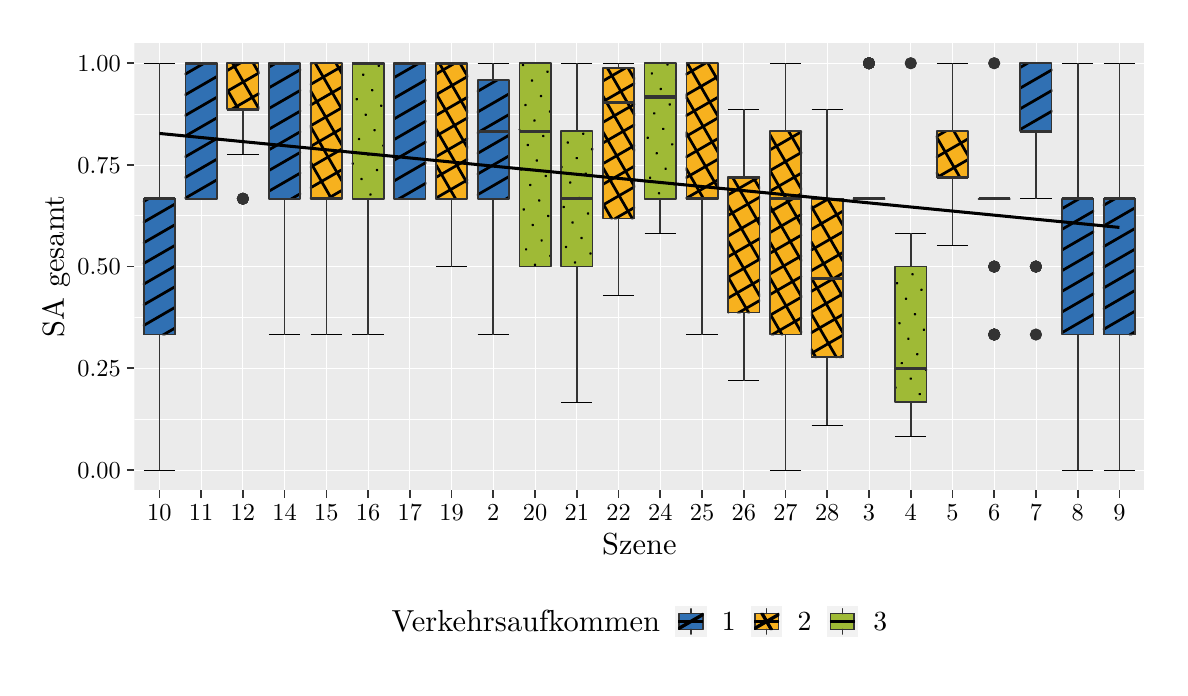
\begin{tikzpicture}[x=1pt,y=1pt]
\definecolor{fillColor}{RGB}{255,255,255}
\path[use as bounding box,fill=fillColor,fill opacity=0.00] (0,0) rectangle (409.05,231.26);
\begin{scope}
\path[clip] (  0.00,  0.00) rectangle (409.05,231.26);
\definecolor{drawColor}{RGB}{255,255,255}
\definecolor{fillColor}{RGB}{255,255,255}

\path[draw=drawColor,line width= 0.6pt,line join=round,line cap=round,fill=fillColor] (  0.00,  0.00) rectangle (409.05,231.26);
\end{scope}
\begin{scope}
\path[clip] ( 38.56, 64.07) rectangle (403.55,225.76);
\definecolor{fillColor}{gray}{0.92}

\path[fill=fillColor] ( 38.56, 64.07) rectangle (403.55,225.76);
\definecolor{drawColor}{RGB}{255,255,255}

\path[draw=drawColor,line width= 0.3pt,line join=round] ( 38.56, 89.79) --
	(403.55, 89.79);

\path[draw=drawColor,line width= 0.3pt,line join=round] ( 38.56,126.54) --
	(403.55,126.54);

\path[draw=drawColor,line width= 0.3pt,line join=round] ( 38.56,163.29) --
	(403.55,163.29);

\path[draw=drawColor,line width= 0.3pt,line join=round] ( 38.56,200.04) --
	(403.55,200.04);

\path[draw=drawColor,line width= 0.3pt,line join=round] ( 38.56, 71.42) --
	(403.55, 71.42);

\path[draw=drawColor,line width= 0.3pt,line join=round] ( 38.56,108.17) --
	(403.55,108.17);

\path[draw=drawColor,line width= 0.3pt,line join=round] ( 38.56,144.92) --
	(403.55,144.92);

\path[draw=drawColor,line width= 0.3pt,line join=round] ( 38.56,181.66) --
	(403.55,181.66);

\path[draw=drawColor,line width= 0.3pt,line join=round] ( 38.56,218.41) --
	(403.55,218.41);

\path[draw=drawColor,line width= 0.3pt,line join=round] ( 47.60, 64.07) --
	( 47.60,225.76);

\path[draw=drawColor,line width= 0.3pt,line join=round] ( 62.69, 64.07) --
	( 62.69,225.76);

\path[draw=drawColor,line width= 0.3pt,line join=round] ( 77.77, 64.07) --
	( 77.77,225.76);

\path[draw=drawColor,line width= 0.3pt,line join=round] ( 92.85, 64.07) --
	( 92.85,225.76);

\path[draw=drawColor,line width= 0.3pt,line join=round] (107.93, 64.07) --
	(107.93,225.76);

\path[draw=drawColor,line width= 0.3pt,line join=round] (123.02, 64.07) --
	(123.02,225.76);

\path[draw=drawColor,line width= 0.3pt,line join=round] (138.10, 64.07) --
	(138.10,225.76);

\path[draw=drawColor,line width= 0.3pt,line join=round] (153.18, 64.07) --
	(153.18,225.76);

\path[draw=drawColor,line width= 0.3pt,line join=round] (168.26, 64.07) --
	(168.26,225.76);

\path[draw=drawColor,line width= 0.3pt,line join=round] (183.35, 64.07) --
	(183.35,225.76);

\path[draw=drawColor,line width= 0.3pt,line join=round] (198.43, 64.07) --
	(198.43,225.76);

\path[draw=drawColor,line width= 0.3pt,line join=round] (213.51, 64.07) --
	(213.51,225.76);

\path[draw=drawColor,line width= 0.3pt,line join=round] (228.59, 64.07) --
	(228.59,225.76);

\path[draw=drawColor,line width= 0.3pt,line join=round] (243.68, 64.07) --
	(243.68,225.76);

\path[draw=drawColor,line width= 0.3pt,line join=round] (258.76, 64.07) --
	(258.76,225.76);

\path[draw=drawColor,line width= 0.3pt,line join=round] (273.84, 64.07) --
	(273.84,225.76);

\path[draw=drawColor,line width= 0.3pt,line join=round] (288.92, 64.07) --
	(288.92,225.76);

\path[draw=drawColor,line width= 0.3pt,line join=round] (304.00, 64.07) --
	(304.00,225.76);

\path[draw=drawColor,line width= 0.3pt,line join=round] (319.09, 64.07) --
	(319.09,225.76);

\path[draw=drawColor,line width= 0.3pt,line join=round] (334.17, 64.07) --
	(334.17,225.76);

\path[draw=drawColor,line width= 0.3pt,line join=round] (349.25, 64.07) --
	(349.25,225.76);

\path[draw=drawColor,line width= 0.3pt,line join=round] (364.33, 64.07) --
	(364.33,225.76);

\path[draw=drawColor,line width= 0.3pt,line join=round] (379.42, 64.07) --
	(379.42,225.76);

\path[draw=drawColor,line width= 0.3pt,line join=round] (394.50, 64.07) --
	(394.50,225.76);
\definecolor{drawColor}{RGB}{0,0,0}

\path[draw=drawColor,line width= 0.2pt,line join=round] ( 41.95,218.41) --
	( 53.26,218.41);

\path[draw=drawColor,line width= 0.2pt,line join=round] ( 47.60,218.41) --
	( 47.60, 71.42);

\path[draw=drawColor,line width= 0.2pt,line join=round] ( 41.95, 71.42) --
	( 53.26, 71.42);

\path[draw=drawColor,line width= 0.2pt,line join=round] ( 57.03,218.41) --
	( 68.34,218.41);

\path[draw=drawColor,line width= 0.2pt,line join=round] ( 62.69,218.41) --
	( 62.69,169.46);

\path[draw=drawColor,line width= 0.2pt,line join=round] ( 57.03,169.46) --
	( 68.34,169.46);

\path[draw=drawColor,line width= 0.2pt,line join=round] ( 72.11,218.41) --
	( 83.43,218.41);

\path[draw=drawColor,line width= 0.2pt,line join=round] ( 77.77,218.41) --
	( 77.77,185.63);

\path[draw=drawColor,line width= 0.2pt,line join=round] ( 72.11,185.63) --
	( 83.43,185.63);

\path[draw=drawColor,line width= 0.2pt,line join=round] ( 87.20,218.41) --
	( 98.51,218.41);

\path[draw=drawColor,line width= 0.2pt,line join=round] ( 92.85,218.41) --
	( 92.85,120.37);

\path[draw=drawColor,line width= 0.2pt,line join=round] ( 87.20,120.37) --
	( 98.51,120.37);

\path[draw=drawColor,line width= 0.2pt,line join=round] (102.28,218.41) --
	(113.59,218.41);

\path[draw=drawColor,line width= 0.2pt,line join=round] (107.93,218.41) --
	(107.93,120.37);

\path[draw=drawColor,line width= 0.2pt,line join=round] (102.28,120.37) --
	(113.59,120.37);

\path[draw=drawColor,line width= 0.2pt,line join=round] (117.36,218.41) --
	(128.67,218.41);

\path[draw=drawColor,line width= 0.2pt,line join=round] (123.02,218.41) --
	(123.02,120.37);

\path[draw=drawColor,line width= 0.2pt,line join=round] (117.36,120.37) --
	(128.67,120.37);

\path[draw=drawColor,line width= 0.2pt,line join=round] (132.44,218.41) --
	(143.75,218.41);

\path[draw=drawColor,line width= 0.2pt,line join=round] (138.10,218.41) --
	(138.10,169.46);

\path[draw=drawColor,line width= 0.2pt,line join=round] (132.44,169.46) --
	(143.75,169.46);

\path[draw=drawColor,line width= 0.2pt,line join=round] (147.53,218.41) --
	(158.84,218.41);

\path[draw=drawColor,line width= 0.2pt,line join=round] (153.18,218.41) --
	(153.18,144.92);

\path[draw=drawColor,line width= 0.2pt,line join=round] (147.53,144.92) --
	(158.84,144.92);

\path[draw=drawColor,line width= 0.2pt,line join=round] (162.61,218.41) --
	(173.92,218.41);

\path[draw=drawColor,line width= 0.2pt,line join=round] (168.26,218.41) --
	(168.26,120.37);

\path[draw=drawColor,line width= 0.2pt,line join=round] (162.61,120.37) --
	(173.92,120.37);

\path[draw=drawColor,line width= 0.2pt,line join=round] (177.69,218.41) --
	(189.00,218.41);

\path[draw=drawColor,line width= 0.2pt,line join=round] (183.35,218.41) --
	(183.35,144.92);

\path[draw=drawColor,line width= 0.2pt,line join=round] (177.69,144.92) --
	(189.00,144.92);

\path[draw=drawColor,line width= 0.2pt,line join=round] (192.77,218.41) --
	(204.08,218.41);

\path[draw=drawColor,line width= 0.2pt,line join=round] (198.43,218.41) --
	(198.43, 95.97);

\path[draw=drawColor,line width= 0.2pt,line join=round] (192.77, 95.97) --
	(204.08, 95.97);

\path[draw=drawColor,line width= 0.2pt,line join=round] (207.85,218.41) --
	(219.17,218.41);

\path[draw=drawColor,line width= 0.2pt,line join=round] (213.51,218.41) --
	(213.51,134.63);

\path[draw=drawColor,line width= 0.2pt,line join=round] (207.85,134.63) --
	(219.17,134.63);

\path[draw=drawColor,line width= 0.2pt,line join=round] (222.94,218.41) --
	(234.25,218.41);

\path[draw=drawColor,line width= 0.2pt,line join=round] (228.59,218.41) --
	(228.59,157.12);

\path[draw=drawColor,line width= 0.2pt,line join=round] (222.94,157.12) --
	(234.25,157.12);

\path[draw=drawColor,line width= 0.2pt,line join=round] (238.02,218.41) --
	(249.33,218.41);

\path[draw=drawColor,line width= 0.2pt,line join=round] (243.68,218.41) --
	(243.68,120.37);

\path[draw=drawColor,line width= 0.2pt,line join=round] (238.02,120.37) --
	(249.33,120.37);

\path[draw=drawColor,line width= 0.2pt,line join=round] (253.10,201.80) --
	(264.41,201.80);

\path[draw=drawColor,line width= 0.2pt,line join=round] (258.76,201.80) --
	(258.76,103.76);

\path[draw=drawColor,line width= 0.2pt,line join=round] (253.10,103.76) --
	(264.41,103.76);

\path[draw=drawColor,line width= 0.2pt,line join=round] (268.18,218.41) --
	(279.50,218.41);

\path[draw=drawColor,line width= 0.2pt,line join=round] (273.84,218.41) --
	(273.84, 71.42);

\path[draw=drawColor,line width= 0.2pt,line join=round] (268.18, 71.42) --
	(279.50, 71.42);

\path[draw=drawColor,line width= 0.2pt,line join=round] (283.27,201.80) --
	(294.58,201.80);

\path[draw=drawColor,line width= 0.2pt,line join=round] (288.92,201.80) --
	(288.92, 87.59);

\path[draw=drawColor,line width= 0.2pt,line join=round] (283.27, 87.59) --
	(294.58, 87.59);

\path[draw=drawColor,line width= 0.2pt,line join=round] (298.35,169.46) --
	(309.66,169.46);

\path[draw=drawColor,line width= 0.2pt,line join=round] (304.00,169.46) --
	(304.00,169.46);

\path[draw=drawColor,line width= 0.2pt,line join=round] (298.35,169.46) --
	(309.66,169.46);

\path[draw=drawColor,line width= 0.2pt,line join=round] (313.43,157.12) --
	(324.74,157.12);

\path[draw=drawColor,line width= 0.2pt,line join=round] (319.09,157.12) --
	(319.09, 83.62);

\path[draw=drawColor,line width= 0.2pt,line join=round] (313.43, 83.62) --
	(324.74, 83.62);

\path[draw=drawColor,line width= 0.2pt,line join=round] (328.51,218.41) --
	(339.83,218.41);

\path[draw=drawColor,line width= 0.2pt,line join=round] (334.17,218.41) --
	(334.17,152.71);

\path[draw=drawColor,line width= 0.2pt,line join=round] (328.51,152.71) --
	(339.83,152.71);

\path[draw=drawColor,line width= 0.2pt,line join=round] (343.60,169.46) --
	(354.91,169.46);

\path[draw=drawColor,line width= 0.2pt,line join=round] (349.25,169.46) --
	(349.25,169.46);

\path[draw=drawColor,line width= 0.2pt,line join=round] (343.60,169.46) --
	(354.91,169.46);

\path[draw=drawColor,line width= 0.2pt,line join=round] (358.68,218.41) --
	(369.99,218.41);

\path[draw=drawColor,line width= 0.2pt,line join=round] (364.33,218.41) --
	(364.33,169.46);

\path[draw=drawColor,line width= 0.2pt,line join=round] (358.68,169.46) --
	(369.99,169.46);

\path[draw=drawColor,line width= 0.2pt,line join=round] (373.76,218.41) --
	(385.07,218.41);

\path[draw=drawColor,line width= 0.2pt,line join=round] (379.42,218.41) --
	(379.42, 71.42);

\path[draw=drawColor,line width= 0.2pt,line join=round] (373.76, 71.42) --
	(385.07, 71.42);

\path[draw=drawColor,line width= 0.2pt,line join=round] (388.84,218.41) --
	(400.15,218.41);

\path[draw=drawColor,line width= 0.2pt,line join=round] (394.50,218.41) --
	(394.50, 71.42);

\path[draw=drawColor,line width= 0.2pt,line join=round] (388.84, 71.42) --
	(400.15, 71.42);
\definecolor{drawColor}{gray}{0.20}

\path[draw=drawColor,line width= 0.2pt,line join=round] ( 47.60,169.46) -- ( 47.60,218.41);

\path[draw=drawColor,line width= 0.2pt,line join=round] ( 47.60,120.37) -- ( 47.60, 71.42);
\definecolor{fillColor}{RGB}{48,112,179}

\path[draw=drawColor,line width= 0.2pt,fill=fillColor] ( 41.95,169.46) --
	( 41.95,120.37) --
	( 53.26,120.37) --
	( 53.26,169.46) --
	( 41.95,169.46) --
	cycle;

\path[draw=drawColor,line width= 0.5pt] ( 41.95,169.46) -- ( 53.26,169.46);

\path[draw=drawColor,line width= 0.2pt,line join=round] ( 62.69,218.41) -- ( 62.69,218.41);

\path[draw=drawColor,line width= 0.2pt,line join=round] ( 62.69,169.46) -- ( 62.69,169.46);

\path[draw=drawColor,line width= 0.2pt,fill=fillColor] ( 57.03,218.41) --
	( 57.03,169.46) --
	( 68.34,169.46) --
	( 68.34,218.41) --
	( 57.03,218.41) --
	cycle;

\path[draw=drawColor,line width= 0.5pt] ( 57.03,218.41) -- ( 68.34,218.41);
\definecolor{fillColor}{gray}{0.20}

\path[draw=drawColor,line width= 0.4pt,line join=round,line cap=round,fill=fillColor] ( 77.77,169.46) circle (  1.96);

\path[draw=drawColor,line width= 0.4pt,line join=round,line cap=round,fill=fillColor] ( 77.77,169.46) circle (  1.96);

\path[draw=drawColor,line width= 0.4pt,line join=round,line cap=round,fill=fillColor] ( 77.77,169.46) circle (  1.96);

\path[draw=drawColor,line width= 0.2pt,line join=round] ( 77.77,218.41) -- ( 77.77,218.41);

\path[draw=drawColor,line width= 0.2pt,line join=round] ( 77.77,201.80) -- ( 77.77,185.63);
\definecolor{fillColor}{RGB}{247,177,30}

\path[draw=drawColor,line width= 0.2pt,fill=fillColor] ( 72.11,218.41) --
	( 72.11,201.80) --
	( 83.43,201.80) --
	( 83.43,218.41) --
	( 72.11,218.41) --
	cycle;

\path[draw=drawColor,line width= 0.5pt] ( 72.11,201.80) -- ( 83.43,201.80);

\path[draw=drawColor,line width= 0.2pt,line join=round] ( 92.85,218.41) -- ( 92.85,218.41);

\path[draw=drawColor,line width= 0.2pt,line join=round] ( 92.85,169.46) -- ( 92.85,120.37);
\definecolor{fillColor}{RGB}{48,112,179}

\path[draw=drawColor,line width= 0.2pt,fill=fillColor] ( 87.20,218.41) --
	( 87.20,169.46) --
	( 98.51,169.46) --
	( 98.51,218.41) --
	( 87.20,218.41) --
	cycle;

\path[draw=drawColor,line width= 0.5pt] ( 87.20,218.41) -- ( 98.51,218.41);

\path[draw=drawColor,line width= 0.2pt,line join=round] (107.93,218.41) -- (107.93,218.41);

\path[draw=drawColor,line width= 0.2pt,line join=round] (107.93,169.46) -- (107.93,120.37);
\definecolor{fillColor}{RGB}{247,177,30}

\path[draw=drawColor,line width= 0.2pt,fill=fillColor] (102.28,218.41) --
	(102.28,169.46) --
	(113.59,169.46) --
	(113.59,218.41) --
	(102.28,218.41) --
	cycle;

\path[draw=drawColor,line width= 0.5pt] (102.28,169.46) -- (113.59,169.46);

\path[draw=drawColor,line width= 0.2pt,line join=round] (123.02,218.41) -- (123.02,218.41);

\path[draw=drawColor,line width= 0.2pt,line join=round] (123.02,169.46) -- (123.02,120.37);
\definecolor{fillColor}{RGB}{159,186,54}

\path[draw=drawColor,line width= 0.2pt,fill=fillColor] (117.36,218.41) --
	(117.36,169.46) --
	(128.67,169.46) --
	(128.67,218.41) --
	(117.36,218.41) --
	cycle;

\path[draw=drawColor,line width= 0.5pt] (117.36,218.41) -- (128.67,218.41);

\path[draw=drawColor,line width= 0.2pt,line join=round] (138.10,218.41) -- (138.10,218.41);

\path[draw=drawColor,line width= 0.2pt,line join=round] (138.10,169.46) -- (138.10,169.46);
\definecolor{fillColor}{RGB}{48,112,179}

\path[draw=drawColor,line width= 0.2pt,fill=fillColor] (132.44,218.41) --
	(132.44,169.46) --
	(143.75,169.46) --
	(143.75,218.41) --
	(132.44,218.41) --
	cycle;

\path[draw=drawColor,line width= 0.5pt] (132.44,218.41) -- (143.75,218.41);

\path[draw=drawColor,line width= 0.2pt,line join=round] (153.18,218.41) -- (153.18,218.41);

\path[draw=drawColor,line width= 0.2pt,line join=round] (153.18,169.46) -- (153.18,144.92);
\definecolor{fillColor}{RGB}{247,177,30}

\path[draw=drawColor,line width= 0.2pt,fill=fillColor] (147.53,218.41) --
	(147.53,169.46) --
	(158.84,169.46) --
	(158.84,218.41) --
	(147.53,218.41) --
	cycle;

\path[draw=drawColor,line width= 0.5pt] (147.53,218.41) -- (158.84,218.41);

\path[draw=drawColor,line width= 0.2pt,line join=round] (168.26,212.28) -- (168.26,218.41);

\path[draw=drawColor,line width= 0.2pt,line join=round] (168.26,169.46) -- (168.26,120.37);
\definecolor{fillColor}{RGB}{48,112,179}

\path[draw=drawColor,line width= 0.2pt,fill=fillColor] (162.61,212.28) --
	(162.61,169.46) --
	(173.92,169.46) --
	(173.92,212.28) --
	(162.61,212.28) --
	cycle;

\path[draw=drawColor,line width= 0.5pt] (162.61,193.87) -- (173.92,193.87);

\path[draw=drawColor,line width= 0.2pt,line join=round] (183.35,218.41) -- (183.35,218.41);

\path[draw=drawColor,line width= 0.2pt,line join=round] (183.35,144.92) -- (183.35,144.92);
\definecolor{fillColor}{RGB}{159,186,54}

\path[draw=drawColor,line width= 0.2pt,fill=fillColor] (177.69,218.41) --
	(177.69,144.92) --
	(189.00,144.92) --
	(189.00,218.41) --
	(177.69,218.41) --
	cycle;

\path[draw=drawColor,line width= 0.5pt] (177.69,193.87) -- (189.00,193.87);

\path[draw=drawColor,line width= 0.2pt,line join=round] (198.43,193.87) -- (198.43,218.41);

\path[draw=drawColor,line width= 0.2pt,line join=round] (198.43,144.92) -- (198.43, 95.97);

\path[draw=drawColor,line width= 0.2pt,fill=fillColor] (192.77,193.87) --
	(192.77,144.92) --
	(204.08,144.92) --
	(204.08,193.87) --
	(192.77,193.87) --
	cycle;

\path[draw=drawColor,line width= 0.5pt] (192.77,169.46) -- (204.08,169.46);

\path[draw=drawColor,line width= 0.2pt,line join=round] (213.51,216.69) -- (213.51,218.41);

\path[draw=drawColor,line width= 0.2pt,line join=round] (213.51,162.30) -- (213.51,134.63);
\definecolor{fillColor}{RGB}{247,177,30}

\path[draw=drawColor,line width= 0.2pt,fill=fillColor] (207.85,216.69) --
	(207.85,162.30) --
	(219.17,162.30) --
	(219.17,216.69) --
	(207.85,216.69) --
	cycle;

\path[draw=drawColor,line width= 0.5pt] (207.85,204.16) -- (219.17,204.16);

\path[draw=drawColor,line width= 0.2pt,line join=round] (228.59,218.41) -- (228.59,218.41);

\path[draw=drawColor,line width= 0.2pt,line join=round] (228.59,169.46) -- (228.59,157.12);
\definecolor{fillColor}{RGB}{159,186,54}

\path[draw=drawColor,line width= 0.2pt,fill=fillColor] (222.94,218.41) --
	(222.94,169.46) --
	(234.25,169.46) --
	(234.25,218.41) --
	(222.94,218.41) --
	cycle;

\path[draw=drawColor,line width= 0.5pt] (222.94,206.21) -- (234.25,206.21);

\path[draw=drawColor,line width= 0.2pt,line join=round] (243.68,218.41) -- (243.68,218.41);

\path[draw=drawColor,line width= 0.2pt,line join=round] (243.68,169.46) -- (243.68,120.37);
\definecolor{fillColor}{RGB}{247,177,30}

\path[draw=drawColor,line width= 0.2pt,fill=fillColor] (238.02,218.41) --
	(238.02,169.46) --
	(249.33,169.46) --
	(249.33,218.41) --
	(238.02,218.41) --
	cycle;

\path[draw=drawColor,line width= 0.5pt] (238.02,169.46) -- (249.33,169.46);

\path[draw=drawColor,line width= 0.2pt,line join=round] (258.76,177.25) -- (258.76,201.80);

\path[draw=drawColor,line width= 0.2pt,line join=round] (258.76,128.30) -- (258.76,103.76);

\path[draw=drawColor,line width= 0.2pt,fill=fillColor] (253.10,177.25) --
	(253.10,128.30) --
	(264.41,128.30) --
	(264.41,177.25) --
	(253.10,177.25) --
	cycle;

\path[draw=drawColor,line width= 0.5pt] (253.10,177.25) -- (264.41,177.25);

\path[draw=drawColor,line width= 0.2pt,line join=round] (273.84,193.87) -- (273.84,218.41);

\path[draw=drawColor,line width= 0.2pt,line join=round] (273.84,120.37) -- (273.84, 71.42);

\path[draw=drawColor,line width= 0.2pt,fill=fillColor] (268.18,193.87) --
	(268.18,120.37) --
	(279.50,120.37) --
	(279.50,193.87) --
	(268.18,193.87) --
	cycle;

\path[draw=drawColor,line width= 0.5pt] (268.18,169.46) -- (279.50,169.46);

\path[draw=drawColor,line width= 0.2pt,line join=round] (288.92,169.46) -- (288.92,201.80);

\path[draw=drawColor,line width= 0.2pt,line join=round] (288.92,112.14) -- (288.92, 87.59);

\path[draw=drawColor,line width= 0.2pt,fill=fillColor] (283.27,169.46) --
	(283.27,112.14) --
	(294.58,112.14) --
	(294.58,169.46) --
	(283.27,169.46) --
	cycle;

\path[draw=drawColor,line width= 0.5pt] (283.27,140.73) -- (294.58,140.73);
\definecolor{fillColor}{gray}{0.20}

\path[draw=drawColor,line width= 0.4pt,line join=round,line cap=round,fill=fillColor] (304.00,218.41) circle (  1.96);

\path[draw=drawColor,line width= 0.4pt,line join=round,line cap=round,fill=fillColor] (304.00,218.41) circle (  1.96);

\path[draw=drawColor,line width= 0.4pt,line join=round,line cap=round,fill=fillColor] (304.00,218.41) circle (  1.96);

\path[draw=drawColor,line width= 0.4pt,line join=round,line cap=round,fill=fillColor] (304.00,218.41) circle (  1.96);

\path[draw=drawColor,line width= 0.4pt,line join=round,line cap=round,fill=fillColor] (304.00,218.41) circle (  1.96);

\path[draw=drawColor,line width= 0.4pt,line join=round,line cap=round,fill=fillColor] (304.00,218.41) circle (  1.96);

\path[draw=drawColor,line width= 0.2pt,line join=round] (304.00,169.46) -- (304.00,169.46);

\path[draw=drawColor,line width= 0.2pt,line join=round] (304.00,169.46) -- (304.00,169.46);
\definecolor{fillColor}{RGB}{48,112,179}

\path[draw=drawColor,line width= 0.2pt,fill=fillColor] (298.35,169.46) --
	(298.35,169.46) --
	(309.66,169.46) --
	(309.66,169.46) --
	(298.35,169.46) --
	cycle;

\path[draw=drawColor,line width= 0.5pt] (298.35,169.46) -- (309.66,169.46);
\definecolor{fillColor}{gray}{0.20}

\path[draw=drawColor,line width= 0.4pt,line join=round,line cap=round,fill=fillColor] (319.09,218.41) circle (  1.96);

\path[draw=drawColor,line width= 0.2pt,line join=round] (319.09,144.92) -- (319.09,157.12);

\path[draw=drawColor,line width= 0.2pt,line join=round] (319.09, 95.97) -- (319.09, 83.62);
\definecolor{fillColor}{RGB}{159,186,54}

\path[draw=drawColor,line width= 0.2pt,fill=fillColor] (313.43,144.92) --
	(313.43, 95.97) --
	(324.74, 95.97) --
	(324.74,144.92) --
	(313.43,144.92) --
	cycle;

\path[draw=drawColor,line width= 0.5pt] (313.43,108.17) -- (324.74,108.17);

\path[draw=drawColor,line width= 0.2pt,line join=round] (334.17,193.87) -- (334.17,218.41);

\path[draw=drawColor,line width= 0.2pt,line join=round] (334.17,177.25) -- (334.17,152.71);
\definecolor{fillColor}{RGB}{247,177,30}

\path[draw=drawColor,line width= 0.2pt,fill=fillColor] (328.51,193.87) --
	(328.51,177.25) --
	(339.83,177.25) --
	(339.83,193.87) --
	(328.51,193.87) --
	cycle;

\path[draw=drawColor,line width= 0.5pt] (328.51,177.25) -- (339.83,177.25);
\definecolor{fillColor}{gray}{0.20}

\path[draw=drawColor,line width= 0.4pt,line join=round,line cap=round,fill=fillColor] (349.25,120.37) circle (  1.96);

\path[draw=drawColor,line width= 0.4pt,line join=round,line cap=round,fill=fillColor] (349.25,144.92) circle (  1.96);

\path[draw=drawColor,line width= 0.4pt,line join=round,line cap=round,fill=fillColor] (349.25,120.37) circle (  1.96);

\path[draw=drawColor,line width= 0.4pt,line join=round,line cap=round,fill=fillColor] (349.25,120.37) circle (  1.96);

\path[draw=drawColor,line width= 0.4pt,line join=round,line cap=round,fill=fillColor] (349.25,144.92) circle (  1.96);

\path[draw=drawColor,line width= 0.4pt,line join=round,line cap=round,fill=fillColor] (349.25,218.41) circle (  1.96);

\path[draw=drawColor,line width= 0.4pt,line join=round,line cap=round,fill=fillColor] (349.25,144.92) circle (  1.96);

\path[draw=drawColor,line width= 0.4pt,line join=round,line cap=round,fill=fillColor] (349.25,120.37) circle (  1.96);

\path[draw=drawColor,line width= 0.2pt,line join=round] (349.25,169.46) -- (349.25,169.46);

\path[draw=drawColor,line width= 0.2pt,line join=round] (349.25,169.46) -- (349.25,169.46);
\definecolor{fillColor}{RGB}{48,112,179}

\path[draw=drawColor,line width= 0.2pt,fill=fillColor] (343.60,169.46) --
	(343.60,169.46) --
	(354.91,169.46) --
	(354.91,169.46) --
	(343.60,169.46) --
	cycle;

\path[draw=drawColor,line width= 0.5pt] (343.60,169.46) -- (354.91,169.46);
\definecolor{fillColor}{gray}{0.20}

\path[draw=drawColor,line width= 0.4pt,line join=round,line cap=round,fill=fillColor] (364.33,144.92) circle (  1.96);

\path[draw=drawColor,line width= 0.4pt,line join=round,line cap=round,fill=fillColor] (364.33,120.37) circle (  1.96);

\path[draw=drawColor,line width= 0.4pt,line join=round,line cap=round,fill=fillColor] (364.33,144.92) circle (  1.96);

\path[draw=drawColor,line width= 0.4pt,line join=round,line cap=round,fill=fillColor] (364.33,144.92) circle (  1.96);

\path[draw=drawColor,line width= 0.2pt,line join=round] (364.33,218.41) -- (364.33,218.41);

\path[draw=drawColor,line width= 0.2pt,line join=round] (364.33,193.87) -- (364.33,169.46);
\definecolor{fillColor}{RGB}{48,112,179}

\path[draw=drawColor,line width= 0.2pt,fill=fillColor] (358.68,218.41) --
	(358.68,193.87) --
	(369.99,193.87) --
	(369.99,218.41) --
	(358.68,218.41) --
	cycle;

\path[draw=drawColor,line width= 0.5pt] (358.68,193.87) -- (369.99,193.87);

\path[draw=drawColor,line width= 0.2pt,line join=round] (379.42,169.46) -- (379.42,218.41);

\path[draw=drawColor,line width= 0.2pt,line join=round] (379.42,120.37) -- (379.42, 71.42);

\path[draw=drawColor,line width= 0.2pt,fill=fillColor] (373.76,169.46) --
	(373.76,120.37) --
	(385.07,120.37) --
	(385.07,169.46) --
	(373.76,169.46) --
	cycle;

\path[draw=drawColor,line width= 0.5pt] (373.76,169.46) -- (385.07,169.46);

\path[draw=drawColor,line width= 0.2pt,line join=round] (394.50,169.46) -- (394.50,218.41);

\path[draw=drawColor,line width= 0.2pt,line join=round] (394.50,120.37) -- (394.50, 71.42);

\path[draw=drawColor,line width= 0.2pt,fill=fillColor] (388.84,169.46) --
	(388.84,120.37) --
	(400.15,120.37) --
	(400.15,169.46) --
	(388.84,169.46) --
	cycle;

\path[draw=drawColor,line width= 0.5pt] (388.84,169.46) -- (400.15,169.46);

\path[draw=drawColor,line width= 0.6pt,line join=round] ( 47.60,169.46) -- ( 47.60,218.41);

\path[draw=drawColor,line width= 0.6pt,line join=round] ( 47.60,120.37) -- ( 47.60, 71.42);

\path[fill=fillColor] ( 41.95,169.46) --
	( 41.95,120.37) --
	( 53.26,120.37) --
	( 53.26,169.46) --
	( 41.95,169.46) --
	cycle;
\definecolor{drawColor}{RGB}{0,0,0}
\definecolor{fillColor}{RGB}{0,0,0}

\path[draw=drawColor,line width= 0.6pt,line join=round,line cap=rect,fill=fillColor] ( 53.26,122.95) --
	( 53.26,122.50) --
	( 49.56,120.37) --
	( 48.79,120.37) --
	( 53.26,122.95) --
	cycle;

\path[draw=drawColor,line width= 0.6pt,line join=round,line cap=rect,fill=fillColor] ( 53.26,130.42) --
	( 53.26,129.97) --
	( 41.95,123.44) --
	( 41.95,123.89) --
	( 53.26,130.42) --
	cycle;

\path[draw=drawColor,line width= 0.6pt,line join=round,line cap=rect,fill=fillColor] ( 53.26,137.89) --
	( 53.26,137.44) --
	( 41.95,130.91) --
	( 41.95,131.36) --
	( 53.26,137.89) --
	cycle;

\path[draw=drawColor,line width= 0.6pt,line join=round,line cap=rect,fill=fillColor] ( 53.26,145.36) --
	( 53.26,144.91) --
	( 41.95,138.38) --
	( 41.95,138.82) --
	( 53.26,145.36) --
	cycle;

\path[draw=drawColor,line width= 0.6pt,line join=round,line cap=rect,fill=fillColor] ( 53.26,152.82) --
	( 53.26,152.38) --
	( 41.95,145.84) --
	( 41.95,146.29) --
	( 53.26,152.82) --
	cycle;

\path[draw=drawColor,line width= 0.6pt,line join=round,line cap=rect,fill=fillColor] ( 53.26,160.29) --
	( 53.26,159.84) --
	( 41.95,153.31) --
	( 41.95,153.76) --
	( 53.26,160.29) --
	cycle;

\path[draw=drawColor,line width= 0.6pt,line join=round,line cap=rect,fill=fillColor] ( 53.26,167.76) --
	( 53.26,167.31) --
	( 41.95,160.78) --
	( 41.95,161.23) --
	( 53.26,167.76) --
	cycle;

\path[draw=drawColor,line width= 0.6pt,line join=round,line cap=rect,fill=fillColor] ( 43.27,169.46) --
	( 44.05,169.46) --
	( 41.95,168.25) --
	( 41.95,168.70) --
	( 43.27,169.46) --
	cycle;
\definecolor{drawColor}{gray}{0.20}

\path[draw=drawColor,line width= 0.6pt,line join=round,line cap=round] ( 41.95,169.46) --
	( 41.95,120.37) --
	( 53.26,120.37) --
	( 53.26,169.46) --
	( 41.95,169.46) --
	cycle;

\path[draw=drawColor,line width= 1.1pt,line join=round] ( 41.95,169.46) -- ( 53.26,169.46);

\path[draw=drawColor,line width= 0.6pt,line join=round] ( 62.69,218.41) -- ( 62.69,218.41);

\path[draw=drawColor,line width= 0.6pt,line join=round] ( 62.69,169.46) -- ( 62.69,169.46);
\definecolor{fillColor}{RGB}{48,112,179}

\path[fill=fillColor] ( 57.03,218.41) --
	( 57.03,169.46) --
	( 68.34,169.46) --
	( 68.34,218.41) --
	( 57.03,218.41) --
	cycle;
\definecolor{drawColor}{RGB}{0,0,0}
\definecolor{fillColor}{RGB}{0,0,0}

\path[draw=drawColor,line width= 0.6pt,line join=round,line cap=rect,fill=fillColor] ( 68.34,176.47) --
	( 68.34,176.02) --
	( 57.03,169.49) --
	( 57.03,169.94) --
	( 68.34,176.47) --
	cycle;

\path[draw=drawColor,line width= 0.6pt,line join=round,line cap=rect,fill=fillColor] ( 68.34,183.94) --
	( 68.34,183.49) --
	( 57.03,176.96) --
	( 57.03,177.41) --
	( 68.34,183.94) --
	cycle;

\path[draw=drawColor,line width= 0.6pt,line join=round,line cap=rect,fill=fillColor] ( 68.34,191.41) --
	( 68.34,190.96) --
	( 57.03,184.43) --
	( 57.03,184.87) --
	( 68.34,191.41) --
	cycle;

\path[draw=drawColor,line width= 0.6pt,line join=round,line cap=rect,fill=fillColor] ( 68.34,198.87) --
	( 68.34,198.43) --
	( 57.03,191.89) --
	( 57.03,192.34) --
	( 68.34,198.87) --
	cycle;

\path[draw=drawColor,line width= 0.6pt,line join=round,line cap=rect,fill=fillColor] ( 68.34,206.34) --
	( 68.34,205.89) --
	( 57.03,199.36) --
	( 57.03,199.81) --
	( 68.34,206.34) --
	cycle;

\path[draw=drawColor,line width= 0.6pt,line join=round,line cap=rect,fill=fillColor] ( 68.34,213.81) --
	( 68.34,213.36) --
	( 57.03,206.83) --
	( 57.03,207.28) --
	( 68.34,213.81) --
	cycle;

\path[draw=drawColor,line width= 0.6pt,line join=round,line cap=rect,fill=fillColor] ( 63.38,218.41) --
	( 64.16,218.41) --
	( 57.03,214.30) --
	( 57.03,214.75) --
	( 63.38,218.41) --
	cycle;
\definecolor{drawColor}{gray}{0.20}

\path[draw=drawColor,line width= 0.6pt,line join=round,line cap=round] ( 57.03,218.41) --
	( 57.03,169.46) --
	( 68.34,169.46) --
	( 68.34,218.41) --
	( 57.03,218.41) --
	cycle;

\path[draw=drawColor,line width= 1.1pt,line join=round] ( 57.03,218.41) -- ( 68.34,218.41);

\path[draw=drawColor,line width= 0.6pt,line join=round] ( 92.85,218.41) -- ( 92.85,218.41);

\path[draw=drawColor,line width= 0.6pt,line join=round] ( 92.85,169.46) -- ( 92.85,120.37);
\definecolor{fillColor}{RGB}{48,112,179}

\path[fill=fillColor] ( 87.20,218.41) --
	( 87.20,169.46) --
	( 98.51,169.46) --
	( 98.51,218.41) --
	( 87.20,218.41) --
	cycle;
\definecolor{drawColor}{RGB}{0,0,0}
\definecolor{fillColor}{RGB}{0,0,0}

\path[draw=drawColor,line width= 0.6pt,line join=round,line cap=rect,fill=fillColor] ( 98.51,171.48) --
	( 98.51,171.03) --
	( 95.79,169.46) --
	( 95.02,169.46) --
	( 98.51,171.48) --
	cycle;

\path[draw=drawColor,line width= 0.6pt,line join=round,line cap=rect,fill=fillColor] ( 98.51,178.95) --
	( 98.51,178.50) --
	( 87.20,171.97) --
	( 87.20,172.42) --
	( 98.51,178.95) --
	cycle;

\path[draw=drawColor,line width= 0.6pt,line join=round,line cap=rect,fill=fillColor] ( 98.51,186.42) --
	( 98.51,185.97) --
	( 87.20,179.44) --
	( 87.20,179.88) --
	( 98.51,186.42) --
	cycle;

\path[draw=drawColor,line width= 0.6pt,line join=round,line cap=rect,fill=fillColor] ( 98.51,193.88) --
	( 98.51,193.44) --
	( 87.20,186.91) --
	( 87.20,187.35) --
	( 98.51,193.88) --
	cycle;

\path[draw=drawColor,line width= 0.6pt,line join=round,line cap=rect,fill=fillColor] ( 98.51,201.35) --
	( 98.51,200.90) --
	( 87.20,194.37) --
	( 87.20,194.82) --
	( 98.51,201.35) --
	cycle;

\path[draw=drawColor,line width= 0.6pt,line join=round,line cap=rect,fill=fillColor] ( 98.51,208.82) --
	( 98.51,208.37) --
	( 87.20,201.84) --
	( 87.20,202.29) --
	( 98.51,208.82) --
	cycle;

\path[draw=drawColor,line width= 0.6pt,line join=round,line cap=rect,fill=fillColor] ( 98.51,216.29) --
	( 98.51,215.84) --
	( 87.20,209.31) --
	( 87.20,209.76) --
	( 98.51,216.29) --
	cycle;

\path[draw=drawColor,line width= 0.6pt,line join=round,line cap=rect,fill=fillColor] ( 89.25,218.41) --
	( 90.03,218.41) --
	( 87.20,216.78) --
	( 87.20,217.23) --
	( 89.25,218.41) --
	cycle;
\definecolor{drawColor}{gray}{0.20}

\path[draw=drawColor,line width= 0.6pt,line join=round,line cap=round] ( 87.20,218.41) --
	( 87.20,169.46) --
	( 98.51,169.46) --
	( 98.51,218.41) --
	( 87.20,218.41) --
	cycle;

\path[draw=drawColor,line width= 1.1pt,line join=round] ( 87.20,218.41) -- ( 98.51,218.41);

\path[draw=drawColor,line width= 0.6pt,line join=round] (138.10,218.41) -- (138.10,218.41);

\path[draw=drawColor,line width= 0.6pt,line join=round] (138.10,169.46) -- (138.10,169.46);
\definecolor{fillColor}{RGB}{48,112,179}

\path[fill=fillColor] (132.44,218.41) --
	(132.44,169.46) --
	(143.75,169.46) --
	(143.75,218.41) --
	(132.44,218.41) --
	cycle;
\definecolor{drawColor}{RGB}{0,0,0}
\definecolor{fillColor}{RGB}{0,0,0}

\path[draw=drawColor,line width= 0.6pt,line join=round,line cap=rect,fill=fillColor] (143.75,175.20) --
	(143.75,174.75) --
	(134.60,169.46) --
	(133.83,169.46) --
	(143.75,175.20) --
	cycle;

\path[draw=drawColor,line width= 0.6pt,line join=round,line cap=rect,fill=fillColor] (143.75,182.67) --
	(143.75,182.22) --
	(132.44,175.69) --
	(132.44,176.13) --
	(143.75,182.67) --
	cycle;

\path[draw=drawColor,line width= 0.6pt,line join=round,line cap=rect,fill=fillColor] (143.75,190.13) --
	(143.75,189.69) --
	(132.44,183.15) --
	(132.44,183.60) --
	(143.75,190.13) --
	cycle;

\path[draw=drawColor,line width= 0.6pt,line join=round,line cap=rect,fill=fillColor] (143.75,197.60) --
	(143.75,197.15) --
	(132.44,190.62) --
	(132.44,191.07) --
	(143.75,197.60) --
	cycle;

\path[draw=drawColor,line width= 0.6pt,line join=round,line cap=rect,fill=fillColor] (143.75,205.07) --
	(143.75,204.62) --
	(132.44,198.09) --
	(132.44,198.54) --
	(143.75,205.07) --
	cycle;

\path[draw=drawColor,line width= 0.6pt,line join=round,line cap=rect,fill=fillColor] (143.75,212.54) --
	(143.75,212.09) --
	(132.44,205.56) --
	(132.44,206.01) --
	(143.75,212.54) --
	cycle;

\path[draw=drawColor,line width= 0.6pt,line join=round,line cap=rect,fill=fillColor] (140.99,218.41) --
	(141.77,218.41) --
	(132.44,213.03) --
	(132.44,213.48) --
	(140.99,218.41) --
	cycle;
\definecolor{drawColor}{gray}{0.20}

\path[draw=drawColor,line width= 0.6pt,line join=round,line cap=round] (132.44,218.41) --
	(132.44,169.46) --
	(143.75,169.46) --
	(143.75,218.41) --
	(132.44,218.41) --
	cycle;

\path[draw=drawColor,line width= 1.1pt,line join=round] (132.44,218.41) -- (143.75,218.41);

\path[draw=drawColor,line width= 0.6pt,line join=round] (168.26,212.28) -- (168.26,218.41);

\path[draw=drawColor,line width= 0.6pt,line join=round] (168.26,169.46) -- (168.26,120.37);
\definecolor{fillColor}{RGB}{48,112,179}

\path[fill=fillColor] (162.61,212.28) --
	(162.61,169.46) --
	(173.92,169.46) --
	(173.92,212.28) --
	(162.61,212.28) --
	cycle;
\definecolor{drawColor}{RGB}{0,0,0}
\definecolor{fillColor}{RGB}{0,0,0}

\path[draw=drawColor,line width= 0.6pt,line join=round,line cap=rect,fill=fillColor] (173.92,170.21) --
	(173.92,169.76) --
	(173.41,169.46) --
	(172.63,169.46) --
	(173.92,170.21) --
	cycle;

\path[draw=drawColor,line width= 0.6pt,line join=round,line cap=rect,fill=fillColor] (173.92,177.68) --
	(173.92,177.23) --
	(162.61,170.70) --
	(162.61,171.14) --
	(173.92,177.68) --
	cycle;

\path[draw=drawColor,line width= 0.6pt,line join=round,line cap=rect,fill=fillColor] (173.92,185.14) --
	(173.92,184.70) --
	(162.61,178.16) --
	(162.61,178.61) --
	(173.92,185.14) --
	cycle;

\path[draw=drawColor,line width= 0.6pt,line join=round,line cap=rect,fill=fillColor] (173.92,192.61) --
	(173.92,192.16) --
	(162.61,185.63) --
	(162.61,186.08) --
	(173.92,192.61) --
	cycle;

\path[draw=drawColor,line width= 0.6pt,line join=round,line cap=rect,fill=fillColor] (173.92,200.08) --
	(173.92,199.63) --
	(162.61,193.10) --
	(162.61,193.55) --
	(173.92,200.08) --
	cycle;

\path[draw=drawColor,line width= 0.6pt,line join=round,line cap=rect,fill=fillColor] (173.92,207.55) --
	(173.92,207.10) --
	(162.61,200.57) --
	(162.61,201.02) --
	(173.92,207.55) --
	cycle;

\path[draw=drawColor,line width= 0.6pt,line join=round,line cap=rect,fill=fillColor] (169.17,212.28) --
	(169.95,212.28) --
	(162.61,208.04) --
	(162.61,208.49) --
	(169.17,212.28) --
	cycle;
\definecolor{drawColor}{gray}{0.20}

\path[draw=drawColor,line width= 0.6pt,line join=round,line cap=round] (162.61,212.28) --
	(162.61,169.46) --
	(173.92,169.46) --
	(173.92,212.28) --
	(162.61,212.28) --
	cycle;

\path[draw=drawColor,line width= 1.1pt,line join=round] (162.61,193.87) -- (173.92,193.87);
\definecolor{fillColor}{gray}{0.20}

\path[draw=drawColor,line width= 0.4pt,line join=round,line cap=round,fill=fillColor] (304.00,218.41) circle (  1.96);

\path[draw=drawColor,line width= 0.4pt,line join=round,line cap=round,fill=fillColor] (304.00,218.41) circle (  1.96);

\path[draw=drawColor,line width= 0.4pt,line join=round,line cap=round,fill=fillColor] (304.00,218.41) circle (  1.96);

\path[draw=drawColor,line width= 0.4pt,line join=round,line cap=round,fill=fillColor] (304.00,218.41) circle (  1.96);

\path[draw=drawColor,line width= 0.4pt,line join=round,line cap=round,fill=fillColor] (304.00,218.41) circle (  1.96);

\path[draw=drawColor,line width= 0.4pt,line join=round,line cap=round,fill=fillColor] (304.00,218.41) circle (  1.96);

\path[draw=drawColor,line width= 0.6pt,line join=round] (304.00,169.46) -- (304.00,169.46);

\path[draw=drawColor,line width= 0.6pt,line join=round] (304.00,169.46) -- (304.00,169.46);
\definecolor{fillColor}{RGB}{48,112,179}

\path[fill=fillColor] (298.35,169.46) --
	(298.35,169.46) --
	(309.66,169.46) --
	(309.66,169.46) --
	(298.35,169.46) --
	cycle;

\path[draw=drawColor,line width= 0.6pt,line join=round,line cap=round] (298.35,169.46) --
	(298.35,169.46) --
	(309.66,169.46) --
	(309.66,169.46) --
	(298.35,169.46) --
	cycle;

\path[draw=drawColor,line width= 1.1pt,line join=round] (298.35,169.46) -- (309.66,169.46);
\definecolor{fillColor}{gray}{0.20}

\path[draw=drawColor,line width= 0.4pt,line join=round,line cap=round,fill=fillColor] (349.25,120.37) circle (  1.96);

\path[draw=drawColor,line width= 0.4pt,line join=round,line cap=round,fill=fillColor] (349.25,144.92) circle (  1.96);

\path[draw=drawColor,line width= 0.4pt,line join=round,line cap=round,fill=fillColor] (349.25,120.37) circle (  1.96);

\path[draw=drawColor,line width= 0.4pt,line join=round,line cap=round,fill=fillColor] (349.25,120.37) circle (  1.96);

\path[draw=drawColor,line width= 0.4pt,line join=round,line cap=round,fill=fillColor] (349.25,144.92) circle (  1.96);

\path[draw=drawColor,line width= 0.4pt,line join=round,line cap=round,fill=fillColor] (349.25,218.41) circle (  1.96);

\path[draw=drawColor,line width= 0.4pt,line join=round,line cap=round,fill=fillColor] (349.25,144.92) circle (  1.96);

\path[draw=drawColor,line width= 0.4pt,line join=round,line cap=round,fill=fillColor] (349.25,120.37) circle (  1.96);

\path[draw=drawColor,line width= 0.6pt,line join=round] (349.25,169.46) -- (349.25,169.46);

\path[draw=drawColor,line width= 0.6pt,line join=round] (349.25,169.46) -- (349.25,169.46);
\definecolor{fillColor}{RGB}{48,112,179}

\path[fill=fillColor] (343.60,169.46) --
	(343.60,169.46) --
	(354.91,169.46) --
	(354.91,169.46) --
	(343.60,169.46) --
	cycle;

\path[draw=drawColor,line width= 0.6pt,line join=round,line cap=round] (343.60,169.46) --
	(343.60,169.46) --
	(354.91,169.46) --
	(354.91,169.46) --
	(343.60,169.46) --
	cycle;

\path[draw=drawColor,line width= 1.1pt,line join=round] (343.60,169.46) -- (354.91,169.46);
\definecolor{fillColor}{gray}{0.20}

\path[draw=drawColor,line width= 0.4pt,line join=round,line cap=round,fill=fillColor] (364.33,144.92) circle (  1.96);

\path[draw=drawColor,line width= 0.4pt,line join=round,line cap=round,fill=fillColor] (364.33,120.37) circle (  1.96);

\path[draw=drawColor,line width= 0.4pt,line join=round,line cap=round,fill=fillColor] (364.33,144.92) circle (  1.96);

\path[draw=drawColor,line width= 0.4pt,line join=round,line cap=round,fill=fillColor] (364.33,144.92) circle (  1.96);

\path[draw=drawColor,line width= 0.6pt,line join=round] (364.33,218.41) -- (364.33,218.41);

\path[draw=drawColor,line width= 0.6pt,line join=round] (364.33,193.87) -- (364.33,169.46);
\definecolor{fillColor}{RGB}{48,112,179}

\path[fill=fillColor] (358.68,218.41) --
	(358.68,193.87) --
	(369.99,193.87) --
	(369.99,218.41) --
	(358.68,218.41) --
	cycle;
\definecolor{drawColor}{RGB}{0,0,0}
\definecolor{fillColor}{RGB}{0,0,0}

\path[draw=drawColor,line width= 0.6pt,line join=round,line cap=rect,fill=fillColor] (369.99,201.26) --
	(369.99,200.81) --
	(358.68,194.28) --
	(358.68,194.72) --
	(369.99,201.26) --
	cycle;

\path[draw=drawColor,line width= 0.6pt,line join=round,line cap=rect,fill=fillColor] (369.99,208.72) --
	(369.99,208.28) --
	(358.68,201.74) --
	(358.68,202.19) --
	(369.99,208.72) --
	cycle;

\path[draw=drawColor,line width= 0.6pt,line join=round,line cap=rect,fill=fillColor] (369.99,216.19) --
	(369.99,215.74) --
	(358.68,209.21) --
	(358.68,209.66) --
	(369.99,216.19) --
	cycle;

\path[draw=drawColor,line width= 0.6pt,line join=round,line cap=rect,fill=fillColor] (360.90,218.41) --
	(361.68,218.41) --
	(358.68,216.68) --
	(358.68,217.13) --
	(360.90,218.41) --
	cycle;
\definecolor{drawColor}{gray}{0.20}

\path[draw=drawColor,line width= 0.6pt,line join=round,line cap=round] (358.68,218.41) --
	(358.68,193.87) --
	(369.99,193.87) --
	(369.99,218.41) --
	(358.68,218.41) --
	cycle;

\path[draw=drawColor,line width= 1.1pt,line join=round] (358.68,193.87) -- (369.99,193.87);

\path[draw=drawColor,line width= 0.6pt,line join=round] (379.42,169.46) -- (379.42,218.41);

\path[draw=drawColor,line width= 0.6pt,line join=round] (379.42,120.37) -- (379.42, 71.42);
\definecolor{fillColor}{RGB}{48,112,179}

\path[fill=fillColor] (373.76,169.46) --
	(373.76,120.37) --
	(385.07,120.37) --
	(385.07,169.46) --
	(373.76,169.46) --
	cycle;
\definecolor{drawColor}{RGB}{0,0,0}
\definecolor{fillColor}{RGB}{0,0,0}

\path[draw=drawColor,line width= 0.6pt,line join=round,line cap=rect,fill=fillColor] (385.07,127.81) --
	(385.07,127.36) --
	(373.76,120.83) --
	(373.76,121.28) --
	(385.07,127.81) --
	cycle;

\path[draw=drawColor,line width= 0.6pt,line join=round,line cap=rect,fill=fillColor] (385.07,135.28) --
	(385.07,134.83) --
	(373.76,128.30) --
	(373.76,128.75) --
	(385.07,135.28) --
	cycle;

\path[draw=drawColor,line width= 0.6pt,line join=round,line cap=rect,fill=fillColor] (385.07,142.75) --
	(385.07,142.30) --
	(373.76,135.77) --
	(373.76,136.22) --
	(385.07,142.75) --
	cycle;

\path[draw=drawColor,line width= 0.6pt,line join=round,line cap=rect,fill=fillColor] (385.07,150.22) --
	(385.07,149.77) --
	(373.76,143.24) --
	(373.76,143.68) --
	(385.07,150.22) --
	cycle;

\path[draw=drawColor,line width= 0.6pt,line join=round,line cap=rect,fill=fillColor] (385.07,157.68) --
	(385.07,157.24) --
	(373.76,150.70) --
	(373.76,151.15) --
	(385.07,157.68) --
	cycle;

\path[draw=drawColor,line width= 0.6pt,line join=round,line cap=rect,fill=fillColor] (385.07,165.15) --
	(385.07,164.70) --
	(373.76,158.17) --
	(373.76,158.62) --
	(385.07,165.15) --
	cycle;

\path[draw=drawColor,line width= 0.6pt,line join=round,line cap=rect,fill=fillColor] (379.60,169.46) --
	(380.38,169.46) --
	(373.76,165.64) --
	(373.76,166.09) --
	(379.60,169.46) --
	cycle;
\definecolor{drawColor}{gray}{0.20}

\path[draw=drawColor,line width= 0.6pt,line join=round,line cap=round] (373.76,169.46) --
	(373.76,120.37) --
	(385.07,120.37) --
	(385.07,169.46) --
	(373.76,169.46) --
	cycle;

\path[draw=drawColor,line width= 1.1pt,line join=round] (373.76,169.46) -- (385.07,169.46);

\path[draw=drawColor,line width= 0.6pt,line join=round] (394.50,169.46) -- (394.50,218.41);

\path[draw=drawColor,line width= 0.6pt,line join=round] (394.50,120.37) -- (394.50, 71.42);
\definecolor{fillColor}{RGB}{48,112,179}

\path[fill=fillColor] (388.84,169.46) --
	(388.84,120.37) --
	(400.15,120.37) --
	(400.15,169.46) --
	(388.84,169.46) --
	cycle;
\definecolor{drawColor}{RGB}{0,0,0}
\definecolor{fillColor}{RGB}{0,0,0}

\path[draw=drawColor,line width= 0.6pt,line join=round,line cap=rect,fill=fillColor] (400.15,121.58) --
	(400.15,121.13) --
	(398.83,120.37) --
	(398.05,120.37) --
	(400.15,121.58) --
	cycle;

\path[draw=drawColor,line width= 0.6pt,line join=round,line cap=rect,fill=fillColor] (400.15,129.05) --
	(400.15,128.60) --
	(388.84,122.07) --
	(388.84,122.52) --
	(400.15,129.05) --
	cycle;

\path[draw=drawColor,line width= 0.6pt,line join=round,line cap=rect,fill=fillColor] (400.15,136.52) --
	(400.15,136.07) --
	(388.84,129.54) --
	(388.84,129.99) --
	(400.15,136.52) --
	cycle;

\path[draw=drawColor,line width= 0.6pt,line join=round,line cap=rect,fill=fillColor] (400.15,143.99) --
	(400.15,143.54) --
	(388.84,137.01) --
	(388.84,137.46) --
	(400.15,143.99) --
	cycle;

\path[draw=drawColor,line width= 0.6pt,line join=round,line cap=rect,fill=fillColor] (400.15,151.45) --
	(400.15,151.01) --
	(388.84,144.48) --
	(388.84,144.92) --
	(400.15,151.45) --
	cycle;

\path[draw=drawColor,line width= 0.6pt,line join=round,line cap=rect,fill=fillColor] (400.15,158.92) --
	(400.15,158.47) --
	(388.84,151.94) --
	(388.84,152.39) --
	(400.15,158.92) --
	cycle;

\path[draw=drawColor,line width= 0.6pt,line join=round,line cap=rect,fill=fillColor] (400.15,166.39) --
	(400.15,165.94) --
	(388.84,159.41) --
	(388.84,159.86) --
	(400.15,166.39) --
	cycle;

\path[draw=drawColor,line width= 0.6pt,line join=round,line cap=rect,fill=fillColor] (392.54,169.46) --
	(393.32,169.46) --
	(388.84,166.88) --
	(388.84,167.33) --
	(392.54,169.46) --
	cycle;
\definecolor{drawColor}{gray}{0.20}

\path[draw=drawColor,line width= 0.6pt,line join=round,line cap=round] (388.84,169.46) --
	(388.84,120.37) --
	(400.15,120.37) --
	(400.15,169.46) --
	(388.84,169.46) --
	cycle;

\path[draw=drawColor,line width= 1.1pt,line join=round] (388.84,169.46) -- (400.15,169.46);
\definecolor{fillColor}{gray}{0.20}

\path[draw=drawColor,line width= 0.4pt,line join=round,line cap=round,fill=fillColor] ( 77.77,169.46) circle (  1.96);

\path[draw=drawColor,line width= 0.4pt,line join=round,line cap=round,fill=fillColor] ( 77.77,169.46) circle (  1.96);

\path[draw=drawColor,line width= 0.4pt,line join=round,line cap=round,fill=fillColor] ( 77.77,169.46) circle (  1.96);

\path[draw=drawColor,line width= 0.6pt,line join=round] ( 77.77,218.41) -- ( 77.77,218.41);

\path[draw=drawColor,line width= 0.6pt,line join=round] ( 77.77,201.80) -- ( 77.77,185.63);
\definecolor{fillColor}{RGB}{247,177,30}

\path[fill=fillColor] ( 72.11,218.41) --
	( 72.11,201.80) --
	( 83.43,201.80) --
	( 83.43,218.41) --
	( 72.11,218.41) --
	cycle;
\definecolor{drawColor}{RGB}{0,0,0}
\definecolor{fillColor}{RGB}{0,0,0}

\path[draw=drawColor,line width= 0.6pt,line join=round,line cap=rect,fill=fillColor] ( 83.43,207.58) --
	( 83.43,207.13) --
	( 74.19,201.80) --
	( 73.42,201.80) --
	( 83.43,207.58) --
	cycle;

\path[draw=drawColor,line width= 0.6pt,line join=round,line cap=rect,fill=fillColor] ( 83.43,215.05) --
	( 83.43,214.60) --
	( 72.11,208.07) --
	( 72.11,208.52) --
	( 83.43,215.05) --
	cycle;

\path[draw=drawColor,line width= 0.6pt,line join=round,line cap=rect,fill=fillColor] ( 76.32,218.41) --
	( 77.09,218.41) --
	( 72.11,215.54) --
	( 72.11,215.99) --
	( 76.32,218.41) --
	cycle;

\path[draw=drawColor,line width= 0.6pt,line join=round,line cap=rect,fill=fillColor] ( 76.40,201.80) --
	( 75.96,201.80) --
	( 72.11,208.46) --
	( 72.11,209.24) --
	( 76.40,201.80) --
	cycle;

\path[draw=drawColor,line width= 0.6pt,line join=round,line cap=rect,fill=fillColor] ( 83.43,202.58) --
	( 83.43,201.80) --
	( 83.42,201.80) --
	( 73.83,218.41) --
	( 74.28,218.41) --
	( 83.43,202.58) --
	cycle;

\path[draw=drawColor,line width= 0.6pt,line join=round,line cap=rect,fill=fillColor] ( 83.43,215.51) --
	( 83.43,214.74) --
	( 81.30,218.41) --
	( 81.75,218.41) --
	( 83.43,215.51) --
	cycle;
\definecolor{drawColor}{gray}{0.20}

\path[draw=drawColor,line width= 0.6pt,line join=round,line cap=round] ( 72.11,218.41) --
	( 72.11,201.80) --
	( 83.43,201.80) --
	( 83.43,218.41) --
	( 72.11,218.41) --
	cycle;

\path[draw=drawColor,line width= 1.1pt,line join=round] ( 72.11,201.80) -- ( 83.43,201.80);

\path[draw=drawColor,line width= 0.6pt,line join=round] (107.93,218.41) -- (107.93,218.41);

\path[draw=drawColor,line width= 0.6pt,line join=round] (107.93,169.46) -- (107.93,120.37);
\definecolor{fillColor}{RGB}{247,177,30}

\path[fill=fillColor] (102.28,218.41) --
	(102.28,169.46) --
	(113.59,169.46) --
	(113.59,218.41) --
	(102.28,218.41) --
	cycle;
\definecolor{drawColor}{RGB}{0,0,0}
\definecolor{fillColor}{RGB}{0,0,0}

\path[draw=drawColor,line width= 0.6pt,line join=round,line cap=rect,fill=fillColor] (113.59,172.72) --
	(113.59,172.27) --
	(108.73,169.46) --
	(107.95,169.46) --
	(113.59,172.72) --
	cycle;

\path[draw=drawColor,line width= 0.6pt,line join=round,line cap=rect,fill=fillColor] (113.59,180.19) --
	(113.59,179.74) --
	(102.28,173.21) --
	(102.28,173.66) --
	(113.59,180.19) --
	cycle;

\path[draw=drawColor,line width= 0.6pt,line join=round,line cap=rect,fill=fillColor] (113.59,187.65) --
	(113.59,187.21) --
	(102.28,180.68) --
	(102.28,181.12) --
	(113.59,187.65) --
	cycle;

\path[draw=drawColor,line width= 0.6pt,line join=round,line cap=rect,fill=fillColor] (113.59,195.12) --
	(113.59,194.68) --
	(102.28,188.14) --
	(102.28,188.59) --
	(113.59,195.12) --
	cycle;

\path[draw=drawColor,line width= 0.6pt,line join=round,line cap=rect,fill=fillColor] (113.59,202.59) --
	(113.59,202.14) --
	(102.28,195.61) --
	(102.28,196.06) --
	(113.59,202.59) --
	cycle;

\path[draw=drawColor,line width= 0.6pt,line join=round,line cap=rect,fill=fillColor] (113.59,210.06) --
	(113.59,209.61) --
	(102.28,203.08) --
	(102.28,203.53) --
	(113.59,210.06) --
	cycle;

\path[draw=drawColor,line width= 0.6pt,line join=round,line cap=rect,fill=fillColor] (113.59,217.53) --
	(113.59,217.08) --
	(102.28,210.55) --
	(102.28,211.00) --
	(113.59,217.53) --
	cycle;

\path[draw=drawColor,line width= 0.6pt,line join=round,line cap=rect,fill=fillColor] (102.28,218.02) --
	(102.28,218.41) --
	(102.96,218.41) --
	(102.28,218.02) --
	cycle;

\path[draw=drawColor,line width= 0.6pt,line join=round,line cap=rect,fill=fillColor] (102.54,169.46) --
	(102.28,169.46) --
	(102.28,169.92) --
	(102.54,169.46) --
	cycle;

\path[draw=drawColor,line width= 0.6pt,line join=round,line cap=rect,fill=fillColor] (110.01,169.46) --
	(109.56,169.46) --
	(102.28,182.08) --
	(102.28,182.86) --
	(110.01,169.46) --
	cycle;

\path[draw=drawColor,line width= 0.6pt,line join=round,line cap=rect,fill=fillColor] (113.59,176.20) --
	(113.59,175.43) --
	(102.28,195.02) --
	(102.28,195.80) --
	(113.59,176.20) --
	cycle;

\path[draw=drawColor,line width= 0.6pt,line join=round,line cap=rect,fill=fillColor] (113.59,189.14) --
	(113.59,188.36) --
	(102.28,207.96) --
	(102.28,208.73) --
	(113.59,189.14) --
	cycle;

\path[draw=drawColor,line width= 0.6pt,line join=round,line cap=rect,fill=fillColor] (113.59,202.08) --
	(113.59,201.30) --
	(103.71,218.41) --
	(104.16,218.41) --
	(113.59,202.08) --
	cycle;

\path[draw=drawColor,line width= 0.6pt,line join=round,line cap=rect,fill=fillColor] (113.59,215.01) --
	(113.59,214.23) --
	(111.18,218.41) --
	(111.62,218.41) --
	(113.59,215.01) --
	cycle;
\definecolor{drawColor}{gray}{0.20}

\path[draw=drawColor,line width= 0.6pt,line join=round,line cap=round] (102.28,218.41) --
	(102.28,169.46) --
	(113.59,169.46) --
	(113.59,218.41) --
	(102.28,218.41) --
	cycle;

\path[draw=drawColor,line width= 1.1pt,line join=round] (102.28,169.46) -- (113.59,169.46);

\path[draw=drawColor,line width= 0.6pt,line join=round] (153.18,218.41) -- (153.18,218.41);

\path[draw=drawColor,line width= 0.6pt,line join=round] (153.18,169.46) -- (153.18,144.92);
\definecolor{fillColor}{RGB}{247,177,30}

\path[fill=fillColor] (147.53,218.41) --
	(147.53,169.46) --
	(158.84,169.46) --
	(158.84,218.41) --
	(147.53,218.41) --
	cycle;
\definecolor{drawColor}{RGB}{0,0,0}
\definecolor{fillColor}{RGB}{0,0,0}

\path[draw=drawColor,line width= 0.6pt,line join=round,line cap=rect,fill=fillColor] (158.84,176.44) --
	(158.84,175.99) --
	(147.54,169.46) --
	(147.53,169.46) --
	(147.53,169.91) --
	(158.84,176.44) --
	cycle;

\path[draw=drawColor,line width= 0.6pt,line join=round,line cap=rect,fill=fillColor] (158.84,183.90) --
	(158.84,183.46) --
	(147.53,176.93) --
	(147.53,177.37) --
	(158.84,183.90) --
	cycle;

\path[draw=drawColor,line width= 0.6pt,line join=round,line cap=rect,fill=fillColor] (158.84,191.37) --
	(158.84,190.92) --
	(147.53,184.39) --
	(147.53,184.84) --
	(158.84,191.37) --
	cycle;

\path[draw=drawColor,line width= 0.6pt,line join=round,line cap=rect,fill=fillColor] (158.84,198.84) --
	(158.84,198.39) --
	(147.53,191.86) --
	(147.53,192.31) --
	(158.84,198.84) --
	cycle;

\path[draw=drawColor,line width= 0.6pt,line join=round,line cap=rect,fill=fillColor] (158.84,206.31) --
	(158.84,205.86) --
	(147.53,199.33) --
	(147.53,199.78) --
	(158.84,206.31) --
	cycle;

\path[draw=drawColor,line width= 0.6pt,line join=round,line cap=rect,fill=fillColor] (158.84,213.78) --
	(158.84,213.33) --
	(147.53,206.80) --
	(147.53,207.25) --
	(158.84,213.78) --
	cycle;

\path[draw=drawColor,line width= 0.6pt,line join=round,line cap=rect,fill=fillColor] (153.93,218.41) --
	(154.71,218.41) --
	(147.53,214.27) --
	(147.53,214.72) --
	(153.93,218.41) --
	cycle;

\path[draw=drawColor,line width= 0.6pt,line join=round,line cap=rect,fill=fillColor] (154.82,169.46) --
	(154.38,169.46) --
	(147.53,181.33) --
	(147.53,182.10) --
	(154.82,169.46) --
	cycle;

\path[draw=drawColor,line width= 0.6pt,line join=round,line cap=rect,fill=fillColor] (158.84,175.45) --
	(158.84,174.67) --
	(147.53,194.26) --
	(147.53,195.04) --
	(158.84,175.45) --
	cycle;

\path[draw=drawColor,line width= 0.6pt,line join=round,line cap=rect,fill=fillColor] (158.84,188.38) --
	(158.84,187.61) --
	(147.53,207.20) --
	(147.53,207.98) --
	(158.84,188.38) --
	cycle;

\path[draw=drawColor,line width= 0.6pt,line join=round,line cap=rect,fill=fillColor] (158.84,201.32) --
	(158.84,200.54) --
	(148.52,218.41) --
	(148.97,218.41) --
	(158.84,201.32) --
	cycle;

\path[draw=drawColor,line width= 0.6pt,line join=round,line cap=rect,fill=fillColor] (158.84,214.26) --
	(158.84,213.48) --
	(155.99,218.41) --
	(156.44,218.41) --
	(158.84,214.26) --
	cycle;
\definecolor{drawColor}{gray}{0.20}

\path[draw=drawColor,line width= 0.6pt,line join=round,line cap=round] (147.53,218.41) --
	(147.53,169.46) --
	(158.84,169.46) --
	(158.84,218.41) --
	(147.53,218.41) --
	cycle;

\path[draw=drawColor,line width= 1.1pt,line join=round] (147.53,218.41) -- (158.84,218.41);

\path[draw=drawColor,line width= 0.6pt,line join=round] (213.51,216.69) -- (213.51,218.41);

\path[draw=drawColor,line width= 0.6pt,line join=round] (213.51,162.30) -- (213.51,134.63);
\definecolor{fillColor}{RGB}{247,177,30}

\path[fill=fillColor] (207.85,216.69) --
	(207.85,162.30) --
	(219.17,162.30) --
	(219.17,216.69) --
	(207.85,216.69) --
	cycle;
\definecolor{drawColor}{RGB}{0,0,0}
\definecolor{fillColor}{RGB}{0,0,0}

\path[draw=drawColor,line width= 0.6pt,line join=round,line cap=rect,fill=fillColor] (219.17,166.46) --
	(219.17,166.01) --
	(212.74,162.30) --
	(211.96,162.30) --
	(219.17,166.46) --
	cycle;

\path[draw=drawColor,line width= 0.6pt,line join=round,line cap=rect,fill=fillColor] (219.17,173.92) --
	(219.17,173.48) --
	(207.85,166.95) --
	(207.85,167.39) --
	(219.17,173.92) --
	cycle;

\path[draw=drawColor,line width= 0.6pt,line join=round,line cap=rect,fill=fillColor] (219.17,181.39) --
	(219.17,180.95) --
	(207.85,174.41) --
	(207.85,174.86) --
	(219.17,181.39) --
	cycle;

\path[draw=drawColor,line width= 0.6pt,line join=round,line cap=rect,fill=fillColor] (219.17,188.86) --
	(219.17,188.41) --
	(207.85,181.88) --
	(207.85,182.33) --
	(219.17,188.86) --
	cycle;

\path[draw=drawColor,line width= 0.6pt,line join=round,line cap=rect,fill=fillColor] (219.17,196.33) --
	(219.17,195.88) --
	(207.85,189.35) --
	(207.85,189.80) --
	(219.17,196.33) --
	cycle;

\path[draw=drawColor,line width= 0.6pt,line join=round,line cap=rect,fill=fillColor] (219.17,203.80) --
	(219.17,203.35) --
	(207.85,196.82) --
	(207.85,197.27) --
	(219.17,203.80) --
	cycle;

\path[draw=drawColor,line width= 0.6pt,line join=round,line cap=rect,fill=fillColor] (219.17,211.27) --
	(219.17,210.82) --
	(207.85,204.29) --
	(207.85,204.74) --
	(219.17,211.27) --
	cycle;

\path[draw=drawColor,line width= 0.6pt,line join=round,line cap=rect,fill=fillColor] (215.62,216.69) --
	(216.39,216.69) --
	(207.85,211.76) --
	(207.85,212.20) --
	(215.62,216.69) --
	cycle;

\path[draw=drawColor,line width= 0.6pt,line join=round,line cap=rect,fill=fillColor] (211.24,162.30) --
	(210.79,162.30) --
	(207.85,167.39) --
	(207.85,168.16) --
	(211.24,162.30) --
	cycle;

\path[draw=drawColor,line width= 0.6pt,line join=round,line cap=rect,fill=fillColor] (218.71,162.30) --
	(218.26,162.30) --
	(207.85,180.32) --
	(207.85,181.10) --
	(218.71,162.30) --
	cycle;

\path[draw=drawColor,line width= 0.6pt,line join=round,line cap=rect,fill=fillColor] (219.17,174.44) --
	(219.17,173.66) --
	(207.85,193.26) --
	(207.85,194.03) --
	(219.17,174.44) --
	cycle;

\path[draw=drawColor,line width= 0.6pt,line join=round,line cap=rect,fill=fillColor] (219.17,187.38) --
	(219.17,186.60) --
	(207.85,206.19) --
	(207.85,206.97) --
	(219.17,187.38) --
	cycle;

\path[draw=drawColor,line width= 0.6pt,line join=round,line cap=rect,fill=fillColor] (219.17,200.31) --
	(219.17,199.54) --
	(209.26,216.69) --
	(209.71,216.69) --
	(219.17,200.31) --
	cycle;

\path[draw=drawColor,line width= 0.6pt,line join=round,line cap=rect,fill=fillColor] (219.17,213.25) --
	(219.17,212.47) --
	(216.73,216.69) --
	(217.18,216.69) --
	(219.17,213.25) --
	cycle;
\definecolor{drawColor}{gray}{0.20}

\path[draw=drawColor,line width= 0.6pt,line join=round,line cap=round] (207.85,216.69) --
	(207.85,162.30) --
	(219.17,162.30) --
	(219.17,216.69) --
	(207.85,216.69) --
	cycle;

\path[draw=drawColor,line width= 1.1pt,line join=round] (207.85,204.16) -- (219.17,204.16);

\path[draw=drawColor,line width= 0.6pt,line join=round] (243.68,218.41) -- (243.68,218.41);

\path[draw=drawColor,line width= 0.6pt,line join=round] (243.68,169.46) -- (243.68,120.37);
\definecolor{fillColor}{RGB}{247,177,30}

\path[fill=fillColor] (238.02,218.41) --
	(238.02,169.46) --
	(249.33,169.46) --
	(249.33,218.41) --
	(238.02,218.41) --
	cycle;
\definecolor{drawColor}{RGB}{0,0,0}
\definecolor{fillColor}{RGB}{0,0,0}

\path[draw=drawColor,line width= 0.6pt,line join=round,line cap=rect,fill=fillColor] (249.33,176.40) --
	(249.33,175.96) --
	(238.09,169.46) --
	(238.02,169.46) --
	(238.02,169.87) --
	(249.33,176.40) --
	cycle;

\path[draw=drawColor,line width= 0.6pt,line join=round,line cap=rect,fill=fillColor] (249.33,183.87) --
	(249.33,183.42) --
	(238.02,176.89) --
	(238.02,177.34) --
	(249.33,183.87) --
	cycle;

\path[draw=drawColor,line width= 0.6pt,line join=round,line cap=rect,fill=fillColor] (249.33,191.34) --
	(249.33,190.89) --
	(238.02,184.36) --
	(238.02,184.81) --
	(249.33,191.34) --
	cycle;

\path[draw=drawColor,line width= 0.6pt,line join=round,line cap=rect,fill=fillColor] (249.33,198.81) --
	(249.33,198.36) --
	(238.02,191.83) --
	(238.02,192.28) --
	(249.33,198.81) --
	cycle;

\path[draw=drawColor,line width= 0.6pt,line join=round,line cap=rect,fill=fillColor] (249.33,206.28) --
	(249.33,205.83) --
	(238.02,199.30) --
	(238.02,199.75) --
	(249.33,206.28) --
	cycle;

\path[draw=drawColor,line width= 0.6pt,line join=round,line cap=rect,fill=fillColor] (249.33,213.75) --
	(249.33,213.30) --
	(238.02,206.77) --
	(238.02,207.22) --
	(249.33,213.75) --
	cycle;

\path[draw=drawColor,line width= 0.6pt,line join=round,line cap=rect,fill=fillColor] (244.48,218.41) --
	(245.26,218.41) --
	(238.02,214.24) --
	(238.02,214.68) --
	(244.48,218.41) --
	cycle;

\path[draw=drawColor,line width= 0.6pt,line join=round,line cap=rect,fill=fillColor] (244.44,169.46) --
	(244.00,169.46) --
	(238.02,179.82) --
	(238.02,180.59) --
	(244.44,169.46) --
	cycle;

\path[draw=drawColor,line width= 0.6pt,line join=round,line cap=rect,fill=fillColor] (249.33,173.94) --
	(249.33,173.16) --
	(238.02,192.75) --
	(238.02,193.53) --
	(249.33,173.94) --
	cycle;

\path[draw=drawColor,line width= 0.6pt,line join=round,line cap=rect,fill=fillColor] (249.33,186.87) --
	(249.33,186.10) --
	(238.02,205.69) --
	(238.02,206.47) --
	(249.33,186.87) --
	cycle;

\path[draw=drawColor,line width= 0.6pt,line join=round,line cap=rect,fill=fillColor] (249.33,199.81) --
	(249.33,199.03) --
	(238.14,218.41) --
	(238.59,218.41) --
	(249.33,199.81) --
	cycle;

\path[draw=drawColor,line width= 0.6pt,line join=round,line cap=rect,fill=fillColor] (249.33,212.74) --
	(249.33,211.97) --
	(245.61,218.41) --
	(246.06,218.41) --
	(249.33,212.74) --
	cycle;
\definecolor{drawColor}{gray}{0.20}

\path[draw=drawColor,line width= 0.6pt,line join=round,line cap=round] (238.02,218.41) --
	(238.02,169.46) --
	(249.33,169.46) --
	(249.33,218.41) --
	(238.02,218.41) --
	cycle;

\path[draw=drawColor,line width= 1.1pt,line join=round] (238.02,169.46) -- (249.33,169.46);

\path[draw=drawColor,line width= 0.6pt,line join=round] (258.76,177.25) -- (258.76,201.80);

\path[draw=drawColor,line width= 0.6pt,line join=round] (258.76,128.30) -- (258.76,103.76);
\definecolor{fillColor}{RGB}{247,177,30}

\path[fill=fillColor] (253.10,177.25) --
	(253.10,128.30) --
	(264.41,128.30) --
	(264.41,177.25) --
	(253.10,177.25) --
	cycle;
\definecolor{drawColor}{RGB}{0,0,0}
\definecolor{fillColor}{RGB}{0,0,0}

\path[draw=drawColor,line width= 0.6pt,line join=round,line cap=rect,fill=fillColor] (264.41,132.83) --
	(264.41,132.38) --
	(257.35,128.30) --
	(256.57,128.30) --
	(264.41,132.83) --
	cycle;

\path[draw=drawColor,line width= 0.6pt,line join=round,line cap=rect,fill=fillColor] (264.41,140.30) --
	(264.41,139.85) --
	(253.10,133.32) --
	(253.10,133.77) --
	(264.41,140.30) --
	cycle;

\path[draw=drawColor,line width= 0.6pt,line join=round,line cap=rect,fill=fillColor] (264.41,147.77) --
	(264.41,147.32) --
	(253.10,140.79) --
	(253.10,141.24) --
	(264.41,147.77) --
	cycle;

\path[draw=drawColor,line width= 0.6pt,line join=round,line cap=rect,fill=fillColor] (264.41,155.24) --
	(264.41,154.79) --
	(253.10,148.26) --
	(253.10,148.71) --
	(264.41,155.24) --
	cycle;

\path[draw=drawColor,line width= 0.6pt,line join=round,line cap=rect,fill=fillColor] (264.41,162.71) --
	(264.41,162.26) --
	(253.10,155.73) --
	(253.10,156.18) --
	(264.41,162.71) --
	cycle;

\path[draw=drawColor,line width= 0.6pt,line join=round,line cap=rect,fill=fillColor] (264.41,170.17) --
	(264.41,169.73) --
	(253.10,163.20) --
	(253.10,163.64) --
	(264.41,170.17) --
	cycle;

\path[draw=drawColor,line width= 0.6pt,line join=round,line cap=rect,fill=fillColor] (263.74,177.25) --
	(264.41,177.25) --
	(264.41,177.19) --
	(253.10,170.66) --
	(253.10,171.11) --
	(263.74,177.25) --
	cycle;

\path[draw=drawColor,line width= 0.6pt,line join=round,line cap=rect,fill=fillColor] (253.27,128.30) --
	(253.10,128.30) --
	(253.10,128.60) --
	(253.27,128.30) --
	cycle;

\path[draw=drawColor,line width= 0.6pt,line join=round,line cap=rect,fill=fillColor] (260.74,128.30) --
	(260.29,128.30) --
	(253.10,140.76) --
	(253.10,141.53) --
	(260.74,128.30) --
	cycle;

\path[draw=drawColor,line width= 0.6pt,line join=round,line cap=rect,fill=fillColor] (264.41,134.88) --
	(264.41,134.10) --
	(253.10,153.69) --
	(253.10,154.47) --
	(264.41,134.88) --
	cycle;

\path[draw=drawColor,line width= 0.6pt,line join=round,line cap=rect,fill=fillColor] (264.41,147.81) --
	(264.41,147.04) --
	(253.10,166.63) --
	(253.10,167.41) --
	(264.41,147.81) --
	cycle;

\path[draw=drawColor,line width= 0.6pt,line join=round,line cap=rect,fill=fillColor] (264.41,160.75) --
	(264.41,159.97) --
	(254.44,177.25) --
	(254.88,177.25) --
	(264.41,160.75) --
	cycle;

\path[draw=drawColor,line width= 0.6pt,line join=round,line cap=rect,fill=fillColor] (264.41,173.68) --
	(264.41,172.91) --
	(261.90,177.25) --
	(262.35,177.25) --
	(264.41,173.68) --
	cycle;
\definecolor{drawColor}{gray}{0.20}

\path[draw=drawColor,line width= 0.6pt,line join=round,line cap=round] (253.10,177.25) --
	(253.10,128.30) --
	(264.41,128.30) --
	(264.41,177.25) --
	(253.10,177.25) --
	cycle;

\path[draw=drawColor,line width= 1.1pt,line join=round] (253.10,177.25) -- (264.41,177.25);

\path[draw=drawColor,line width= 0.6pt,line join=round] (273.84,193.87) -- (273.84,218.41);

\path[draw=drawColor,line width= 0.6pt,line join=round] (273.84,120.37) -- (273.84, 71.42);
\definecolor{fillColor}{RGB}{247,177,30}

\path[fill=fillColor] (268.18,193.87) --
	(268.18,120.37) --
	(279.50,120.37) --
	(279.50,193.87) --
	(268.18,193.87) --
	cycle;
\definecolor{drawColor}{RGB}{0,0,0}
\definecolor{fillColor}{RGB}{0,0,0}

\path[draw=drawColor,line width= 0.6pt,line join=round,line cap=rect,fill=fillColor] (279.50,126.60) --
	(279.50,126.15) --
	(269.47,120.37) --
	(268.69,120.37) --
	(279.50,126.60) --
	cycle;

\path[draw=drawColor,line width= 0.6pt,line join=round,line cap=rect,fill=fillColor] (279.50,134.07) --
	(279.50,133.62) --
	(268.18,127.09) --
	(268.18,127.54) --
	(279.50,134.07) --
	cycle;

\path[draw=drawColor,line width= 0.6pt,line join=round,line cap=rect,fill=fillColor] (279.50,141.54) --
	(279.50,141.09) --
	(268.18,134.56) --
	(268.18,135.01) --
	(279.50,141.54) --
	cycle;

\path[draw=drawColor,line width= 0.6pt,line join=round,line cap=rect,fill=fillColor] (279.50,149.01) --
	(279.50,148.56) --
	(268.18,142.03) --
	(268.18,142.48) --
	(279.50,149.01) --
	cycle;

\path[draw=drawColor,line width= 0.6pt,line join=round,line cap=rect,fill=fillColor] (279.50,156.48) --
	(279.50,156.03) --
	(268.18,149.50) --
	(268.18,149.95) --
	(279.50,156.48) --
	cycle;

\path[draw=drawColor,line width= 0.6pt,line join=round,line cap=rect,fill=fillColor] (279.50,163.95) --
	(279.50,163.50) --
	(268.18,156.97) --
	(268.18,157.41) --
	(279.50,163.95) --
	cycle;

\path[draw=drawColor,line width= 0.6pt,line join=round,line cap=rect,fill=fillColor] (279.50,171.41) --
	(279.50,170.97) --
	(268.18,164.43) --
	(268.18,164.88) --
	(279.50,171.41) --
	cycle;

\path[draw=drawColor,line width= 0.6pt,line join=round,line cap=rect,fill=fillColor] (279.50,178.88) --
	(279.50,178.43) --
	(268.18,171.90) --
	(268.18,172.35) --
	(279.50,178.88) --
	cycle;

\path[draw=drawColor,line width= 0.6pt,line join=round,line cap=rect,fill=fillColor] (279.50,186.35) --
	(279.50,185.90) --
	(268.18,179.37) --
	(268.18,179.82) --
	(279.50,186.35) --
	cycle;

\path[draw=drawColor,line width= 0.6pt,line join=round,line cap=rect,fill=fillColor] (279.50,193.82) --
	(279.50,193.37) --
	(268.18,186.84) --
	(268.18,187.29) --
	(279.50,193.82) --
	cycle;

\path[draw=drawColor,line width= 0.6pt,line join=round,line cap=rect,fill=fillColor] (272.79,120.37) --
	(272.34,120.37) --
	(268.18,127.57) --
	(268.18,128.35) --
	(272.79,120.37) --
	cycle;

\path[draw=drawColor,line width= 0.6pt,line join=round,line cap=rect,fill=fillColor] (279.50,121.69) --
	(279.50,120.91) --
	(268.18,140.51) --
	(268.18,141.28) --
	(279.50,121.69) --
	cycle;

\path[draw=drawColor,line width= 0.6pt,line join=round,line cap=rect,fill=fillColor] (279.50,134.63) --
	(279.50,133.85) --
	(268.18,153.44) --
	(268.18,154.22) --
	(279.50,134.63) --
	cycle;

\path[draw=drawColor,line width= 0.6pt,line join=round,line cap=rect,fill=fillColor] (279.50,147.56) --
	(279.50,146.79) --
	(268.18,166.38) --
	(268.18,167.15) --
	(279.50,147.56) --
	cycle;

\path[draw=drawColor,line width= 0.6pt,line join=round,line cap=rect,fill=fillColor] (279.50,160.50) --
	(279.50,159.72) --
	(268.18,179.31) --
	(268.18,180.09) --
	(279.50,160.50) --
	cycle;

\path[draw=drawColor,line width= 0.6pt,line join=round,line cap=rect,fill=fillColor] (279.50,173.43) --
	(279.50,172.66) --
	(268.18,192.25) --
	(268.18,193.03) --
	(279.50,173.43) --
	cycle;

\path[draw=drawColor,line width= 0.6pt,line join=round,line cap=rect,fill=fillColor] (279.50,186.37) --
	(279.50,185.59) --
	(274.72,193.87) --
	(275.17,193.87) --
	(279.50,186.37) --
	cycle;
\definecolor{drawColor}{gray}{0.20}

\path[draw=drawColor,line width= 0.6pt,line join=round,line cap=round] (268.18,193.87) --
	(268.18,120.37) --
	(279.50,120.37) --
	(279.50,193.87) --
	(268.18,193.87) --
	cycle;

\path[draw=drawColor,line width= 1.1pt,line join=round] (268.18,169.46) -- (279.50,169.46);

\path[draw=drawColor,line width= 0.6pt,line join=round] (288.92,169.46) -- (288.92,201.80);

\path[draw=drawColor,line width= 0.6pt,line join=round] (288.92,112.14) -- (288.92, 87.59);
\definecolor{fillColor}{RGB}{247,177,30}

\path[fill=fillColor] (283.27,169.46) --
	(283.27,112.14) --
	(294.58,112.14) --
	(294.58,169.46) --
	(283.27,169.46) --
	cycle;
\definecolor{drawColor}{RGB}{0,0,0}
\definecolor{fillColor}{RGB}{0,0,0}

\path[draw=drawColor,line width= 0.6pt,line join=round,line cap=rect,fill=fillColor] (294.58,112.91) --
	(294.58,112.46) --
	(294.02,112.14) --
	(293.24,112.14) --
	(294.58,112.91) --
	cycle;

\path[draw=drawColor,line width= 0.6pt,line join=round,line cap=rect,fill=fillColor] (294.58,120.37) --
	(294.58,119.93) --
	(283.27,113.39) --
	(283.27,113.84) --
	(294.58,120.37) --
	cycle;

\path[draw=drawColor,line width= 0.6pt,line join=round,line cap=rect,fill=fillColor] (294.58,127.84) --
	(294.58,127.39) --
	(283.27,120.86) --
	(283.27,121.31) --
	(294.58,127.84) --
	cycle;

\path[draw=drawColor,line width= 0.6pt,line join=round,line cap=rect,fill=fillColor] (294.58,135.31) --
	(294.58,134.86) --
	(283.27,128.33) --
	(283.27,128.78) --
	(294.58,135.31) --
	cycle;

\path[draw=drawColor,line width= 0.6pt,line join=round,line cap=rect,fill=fillColor] (294.58,142.78) --
	(294.58,142.33) --
	(283.27,135.80) --
	(283.27,136.25) --
	(294.58,142.78) --
	cycle;

\path[draw=drawColor,line width= 0.6pt,line join=round,line cap=rect,fill=fillColor] (294.58,150.25) --
	(294.58,149.80) --
	(283.27,143.27) --
	(283.27,143.72) --
	(294.58,150.25) --
	cycle;

\path[draw=drawColor,line width= 0.6pt,line join=round,line cap=rect,fill=fillColor] (294.58,157.72) --
	(294.58,157.27) --
	(283.27,150.74) --
	(283.27,151.19) --
	(294.58,157.72) --
	cycle;

\path[draw=drawColor,line width= 0.6pt,line join=round,line cap=rect,fill=fillColor] (294.58,165.18) --
	(294.58,164.74) --
	(283.27,158.21) --
	(283.27,158.65) --
	(294.58,165.18) --
	cycle;

\path[draw=drawColor,line width= 0.6pt,line join=round,line cap=rect,fill=fillColor] (289.05,169.46) --
	(289.83,169.46) --
	(283.27,165.67) --
	(283.27,166.12) --
	(289.05,169.46) --
	cycle;

\path[draw=drawColor,line width= 0.6pt,line join=round,line cap=rect,fill=fillColor] (285.01,112.14) --
	(284.56,112.14) --
	(283.27,114.38) --
	(283.27,115.16) --
	(285.01,112.14) --
	cycle;

\path[draw=drawColor,line width= 0.6pt,line join=round,line cap=rect,fill=fillColor] (292.48,112.14) --
	(292.03,112.14) --
	(283.27,127.32) --
	(283.27,128.09) --
	(292.48,112.14) --
	cycle;

\path[draw=drawColor,line width= 0.6pt,line join=round,line cap=rect,fill=fillColor] (294.58,121.44) --
	(294.58,120.66) --
	(283.27,140.25) --
	(283.27,141.03) --
	(294.58,121.44) --
	cycle;

\path[draw=drawColor,line width= 0.6pt,line join=round,line cap=rect,fill=fillColor] (294.58,134.37) --
	(294.58,133.60) --
	(283.27,153.19) --
	(283.27,153.97) --
	(294.58,134.37) --
	cycle;

\path[draw=drawColor,line width= 0.6pt,line join=round,line cap=rect,fill=fillColor] (294.58,147.31) --
	(294.58,146.53) --
	(283.27,166.13) --
	(283.27,166.90) --
	(294.58,147.31) --
	cycle;

\path[draw=drawColor,line width= 0.6pt,line join=round,line cap=rect,fill=fillColor] (294.58,160.25) --
	(294.58,159.47) --
	(288.81,169.46) --
	(289.26,169.46) --
	(294.58,160.25) --
	cycle;
\definecolor{drawColor}{gray}{0.20}

\path[draw=drawColor,line width= 0.6pt,line join=round,line cap=round] (283.27,169.46) --
	(283.27,112.14) --
	(294.58,112.14) --
	(294.58,169.46) --
	(283.27,169.46) --
	cycle;

\path[draw=drawColor,line width= 1.1pt,line join=round] (283.27,140.73) -- (294.58,140.73);

\path[draw=drawColor,line width= 0.6pt,line join=round] (334.17,193.87) -- (334.17,218.41);

\path[draw=drawColor,line width= 0.6pt,line join=round] (334.17,177.25) -- (334.17,152.71);
\definecolor{fillColor}{RGB}{247,177,30}

\path[fill=fillColor] (328.51,193.87) --
	(328.51,177.25) --
	(339.83,177.25) --
	(339.83,193.87) --
	(328.51,193.87) --
	cycle;
\definecolor{drawColor}{RGB}{0,0,0}
\definecolor{fillColor}{RGB}{0,0,0}

\path[draw=drawColor,line width= 0.6pt,line join=round,line cap=rect,fill=fillColor] (339.83,183.84) --
	(339.83,183.39) --
	(329.20,177.25) --
	(328.51,177.25) --
	(328.51,177.31) --
	(339.83,183.84) --
	cycle;

\path[draw=drawColor,line width= 0.6pt,line join=round,line cap=rect,fill=fillColor] (339.83,191.31) --
	(339.83,190.86) --
	(328.51,184.33) --
	(328.51,184.78) --
	(339.83,191.31) --
	cycle;

\path[draw=drawColor,line width= 0.6pt,line join=round,line cap=rect,fill=fillColor] (331.32,193.87) --
	(332.10,193.87) --
	(328.51,191.80) --
	(328.51,192.25) --
	(331.32,193.87) --
	cycle;

\path[draw=drawColor,line width= 0.6pt,line join=round,line cap=rect,fill=fillColor] (329.57,177.25) --
	(329.12,177.25) --
	(328.51,178.31) --
	(328.51,179.08) --
	(329.57,177.25) --
	cycle;

\path[draw=drawColor,line width= 0.6pt,line join=round,line cap=rect,fill=fillColor] (337.04,177.25) --
	(336.59,177.25) --
	(328.51,191.24) --
	(328.51,192.02) --
	(337.04,177.25) --
	cycle;

\path[draw=drawColor,line width= 0.6pt,line join=round,line cap=rect,fill=fillColor] (339.83,185.36) --
	(339.83,184.59) --
	(334.47,193.87) --
	(334.92,193.87) --
	(339.83,185.36) --
	cycle;
\definecolor{drawColor}{gray}{0.20}

\path[draw=drawColor,line width= 0.6pt,line join=round,line cap=round] (328.51,193.87) --
	(328.51,177.25) --
	(339.83,177.25) --
	(339.83,193.87) --
	(328.51,193.87) --
	cycle;

\path[draw=drawColor,line width= 1.1pt,line join=round] (328.51,177.25) -- (339.83,177.25);

\path[draw=drawColor,line width= 0.6pt,line join=round] (123.02,218.41) -- (123.02,218.41);

\path[draw=drawColor,line width= 0.6pt,line join=round] (123.02,169.46) -- (123.02,120.37);
\definecolor{fillColor}{RGB}{159,186,54}

\path[fill=fillColor] (117.36,218.41) --
	(117.36,169.46) --
	(128.67,169.46) --
	(128.67,218.41) --
	(117.36,218.41) --
	cycle;
\definecolor{drawColor}{RGB}{0,0,0}
\definecolor{fillColor}{RGB}{0,0,0}

\path[draw=drawColor,line width= 0.6pt,line join=round,line cap=round,fill=fillColor] (118.90,205.43) circle (  0.19);

\path[draw=drawColor,line width= 0.6pt,line join=round,line cap=round,fill=fillColor] (119.76,190.99) circle (  0.19);

\path[draw=drawColor,line width= 0.6pt,line join=round,line cap=round,fill=fillColor] (120.63,176.56) circle (  0.19);

\path[draw=drawColor,line width= 0.6pt,line join=round,line cap=round,fill=fillColor] (121.26,214.27) circle (  0.19);

\path[draw=drawColor,line width= 0.6pt,line join=round,line cap=round,fill=fillColor] (122.13,199.83) circle (  0.19);

\path[draw=drawColor,line width= 0.6pt,line join=round,line cap=round,fill=fillColor] (123.00,185.39) circle (  0.19);

\path[draw=drawColor,line width= 0.6pt,line join=round,line cap=round,fill=fillColor] (123.86,170.96) circle (  0.19);

\path[draw=drawColor,line width= 0.6pt,line join=round,line cap=round,fill=fillColor] (124.50,208.67) circle (  0.19);

\path[draw=drawColor,line width= 0.6pt,line join=round,line cap=round,fill=fillColor] (125.36,194.23) circle (  0.19);

\path[draw=drawColor,line width= 0.6pt,line join=round,line cap=round,fill=fillColor] (126.23,179.79) circle (  0.19);

\path[draw=drawColor,line width= 0.6pt,line join=round,line cap=round,fill=fillColor] (126.87,217.50) circle (  0.19);

\path[draw=drawColor,line width= 0.6pt,line join=round,line cap=round,fill=fillColor] (127.73,203.06) circle (  0.19);

\path[draw=drawColor,line width= 0.6pt,line join=round,line cap=round,fill=fillColor] (117.37,182.35) --
	(117.38,182.35) --
	(117.39,182.35) --
	(117.40,182.35) --
	(117.42,182.35) --
	(117.43,182.35) --
	(117.44,182.35) --
	(117.45,182.35) --
	(117.46,182.34) --
	(117.47,182.34) --
	(117.49,182.33) --
	(117.50,182.33) --
	(117.51,182.32) --
	(117.52,182.31) --
	(117.53,182.30) --
	(117.53,182.30) --
	(117.54,182.29) --
	(117.55,182.28) --
	(117.56,182.27) --
	(117.56,182.26) --
	(117.57,182.25) --
	(117.57,182.23) --
	(117.58,182.22) --
	(117.58,182.21) --
	(117.59,182.20) --
	(117.59,182.19) --
	(117.59,182.18) --
	(117.59,182.16) --
	(117.59,182.15) --
	(117.59,182.14) --
	(117.59,182.13) --
	(117.58,182.12) --
	(117.58,182.10) --
	(117.58,182.09) --
	(117.57,182.08) --
	(117.57,182.07) --
	(117.56,182.06) --
	(117.55,182.05) --
	(117.55,182.04) --
	(117.54,182.03) --
	(117.53,182.02) --
	(117.52,182.01) --
	(117.51,182.01) --
	(117.50,182.00) --
	(117.49,181.99) --
	(117.48,181.99) --
	(117.47,181.98) --
	(117.46,181.98) --
	(117.45,181.97) --
	(117.44,181.97) --
	(117.42,181.97) --
	(117.41,181.97) --
	(117.40,181.97) --
	(117.39,181.97) --
	(117.38,181.97) --
	(117.36,181.97) --
	(117.36,181.97) --
	(117.36,182.35) --
	(117.37,182.35) --
	cycle;

\path[draw=drawColor,line width= 0.6pt,line join=round,line cap=round,fill=fillColor] (128.66,188.44) --
	(128.65,188.44) --
	(128.64,188.44) --
	(128.63,188.44) --
	(128.61,188.43) --
	(128.60,188.43) --
	(128.59,188.43) --
	(128.58,188.43) --
	(128.57,188.44) --
	(128.55,188.44) --
	(128.54,188.44) --
	(128.53,188.45) --
	(128.52,188.45) --
	(128.51,188.46) --
	(128.50,188.46) --
	(128.49,188.47) --
	(128.48,188.48) --
	(128.47,188.48) --
	(128.46,188.49) --
	(128.45,188.50) --
	(128.44,188.51) --
	(128.44,188.52) --
	(128.43,188.53) --
	(128.42,188.54) --
	(128.42,188.55) --
	(128.41,188.56) --
	(128.41,188.58) --
	(128.41,188.59) --
	(128.41,188.60) --
	(128.40,188.61) --
	(128.40,188.62) --
	(128.40,188.64) --
	(128.41,188.65) --
	(128.41,188.66) --
	(128.41,188.67) --
	(128.41,188.68) --
	(128.42,188.70) --
	(128.42,188.71) --
	(128.43,188.72) --
	(128.43,188.73) --
	(128.44,188.74) --
	(128.45,188.75) --
	(128.45,188.76) --
	(128.46,188.77) --
	(128.47,188.77) --
	(128.48,188.78) --
	(128.49,188.79) --
	(128.50,188.80) --
	(128.51,188.80) --
	(128.52,188.81) --
	(128.53,188.81) --
	(128.55,188.81) --
	(128.56,188.82) --
	(128.57,188.82) --
	(128.58,188.82) --
	(128.59,188.82) --
	(128.61,188.82) --
	(128.62,188.82) --
	(128.63,188.82) --
	(128.64,188.82) --
	(128.65,188.81) --
	(128.67,188.81) --
	(128.67,188.81) --
	(128.67,188.45) --
	(128.66,188.44) --
	cycle;
\definecolor{drawColor}{gray}{0.20}

\path[draw=drawColor,line width= 0.6pt,line join=round,line cap=round] (117.36,218.41) --
	(117.36,169.46) --
	(128.67,169.46) --
	(128.67,218.41) --
	(117.36,218.41) --
	cycle;

\path[draw=drawColor,line width= 1.1pt,line join=round] (117.36,218.41) -- (128.67,218.41);

\path[draw=drawColor,line width= 0.6pt,line join=round] (183.35,218.41) -- (183.35,218.41);

\path[draw=drawColor,line width= 0.6pt,line join=round] (183.35,144.92) -- (183.35,144.92);
\definecolor{fillColor}{RGB}{159,186,54}

\path[fill=fillColor] (177.69,218.41) --
	(177.69,144.92) --
	(189.00,144.92) --
	(189.00,218.41) --
	(177.69,218.41) --
	cycle;
\definecolor{drawColor}{RGB}{0,0,0}
\definecolor{fillColor}{RGB}{0,0,0}

\path[draw=drawColor,line width= 0.6pt,line join=round,line cap=round,fill=fillColor] (178.38,180.02) circle (  0.19);

\path[draw=drawColor,line width= 0.6pt,line join=round,line cap=round,fill=fillColor] (179.01,217.73) circle (  0.19);

\path[draw=drawColor,line width= 0.6pt,line join=round,line cap=round,fill=fillColor] (179.24,165.59) circle (  0.19);

\path[draw=drawColor,line width= 0.6pt,line join=round,line cap=round,fill=fillColor] (179.88,203.30) circle (  0.19);

\path[draw=drawColor,line width= 0.6pt,line join=round,line cap=round,fill=fillColor] (180.11,151.15) circle (  0.19);

\path[draw=drawColor,line width= 0.6pt,line join=round,line cap=round,fill=fillColor] (180.74,188.86) circle (  0.19);

\path[draw=drawColor,line width= 0.6pt,line join=round,line cap=round,fill=fillColor] (181.61,174.42) circle (  0.19);

\path[draw=drawColor,line width= 0.6pt,line join=round,line cap=round,fill=fillColor] (182.24,212.13) circle (  0.19);

\path[draw=drawColor,line width= 0.6pt,line join=round,line cap=round,fill=fillColor] (182.48,159.99) circle (  0.19);

\path[draw=drawColor,line width= 0.6pt,line join=round,line cap=round,fill=fillColor] (183.11,197.70) circle (  0.19);

\path[draw=drawColor,line width= 0.6pt,line join=round,line cap=round,fill=fillColor] (183.34,145.55) circle (  0.19);

\path[draw=drawColor,line width= 0.6pt,line join=round,line cap=round,fill=fillColor] (183.98,183.26) circle (  0.19);

\path[draw=drawColor,line width= 0.6pt,line join=round,line cap=round,fill=fillColor] (184.84,168.82) circle (  0.19);

\path[draw=drawColor,line width= 0.6pt,line join=round,line cap=round,fill=fillColor] (185.48,206.53) circle (  0.19);

\path[draw=drawColor,line width= 0.6pt,line join=round,line cap=round,fill=fillColor] (185.71,154.39) circle (  0.19);

\path[draw=drawColor,line width= 0.6pt,line join=round,line cap=round,fill=fillColor] (186.34,192.09) circle (  0.19);

\path[draw=drawColor,line width= 0.6pt,line join=round,line cap=round,fill=fillColor] (187.21,177.66) circle (  0.19);

\path[draw=drawColor,line width= 0.6pt,line join=round,line cap=round,fill=fillColor] (187.85,215.37) circle (  0.19);

\path[draw=drawColor,line width= 0.6pt,line join=round,line cap=round,fill=fillColor] (188.08,163.22) circle (  0.19);

\path[draw=drawColor,line width= 0.6pt,line join=round,line cap=round,fill=fillColor] (188.71,200.93) circle (  0.19);

\path[draw=drawColor,line width= 0.6pt,line join=round,line cap=round,fill=fillColor] (177.69,194.52) --
	(177.70,194.51) --
	(177.70,194.50) --
	(177.70,194.49) --
	(177.70,194.48) --
	(177.70,194.47) --
	(177.70,194.45) --
	(177.70,194.44) --
	(177.70,194.43) --
	(177.70,194.42) --
	(177.70,194.41) --
	(177.69,194.39) --
	(177.69,194.39) --
	(177.69,194.53) --
	(177.69,194.52) --
	cycle;

\path[draw=drawColor,line width= 0.6pt,line join=round,line cap=round,fill=fillColor] (189.00,148.60) --
	(188.98,148.59) --
	(188.97,148.59) --
	(188.96,148.59) --
	(188.95,148.59) --
	(188.94,148.59) --
	(188.92,148.59) --
	(188.91,148.59) --
	(188.90,148.59) --
	(188.89,148.60) --
	(188.88,148.60) --
	(188.87,148.61) --
	(188.85,148.61) --
	(188.84,148.62) --
	(188.83,148.62) --
	(188.82,148.63) --
	(188.81,148.64) --
	(188.81,148.65) --
	(188.80,148.66) --
	(188.79,148.67) --
	(188.78,148.68) --
	(188.78,148.69) --
	(188.77,148.70) --
	(188.77,148.71) --
	(188.76,148.72) --
	(188.76,148.73) --
	(188.75,148.74) --
	(188.75,148.76) --
	(188.75,148.77) --
	(188.75,148.78) --
	(188.75,148.79) --
	(188.75,148.80) --
	(188.75,148.82) --
	(188.76,148.83) --
	(188.76,148.84) --
	(188.76,148.85) --
	(188.77,148.86) --
	(188.77,148.87) --
	(188.78,148.88) --
	(188.79,148.89) --
	(188.79,148.90) --
	(188.80,148.91) --
	(188.81,148.92) --
	(188.82,148.93) --
	(188.83,148.94) --
	(188.84,148.95) --
	(188.85,148.95) --
	(188.86,148.96) --
	(188.87,148.96) --
	(188.88,148.97) --
	(188.89,148.97) --
	(188.90,148.97) --
	(188.92,148.98) --
	(188.93,148.98) --
	(188.94,148.98) --
	(188.95,148.98) --
	(188.96,148.98) --
	(188.98,148.98) --
	(188.99,148.97) --
	(189.00,148.97) --
	(189.00,148.97) --
	(189.00,148.60) --
	(189.00,148.60) --
	cycle;
\definecolor{drawColor}{gray}{0.20}

\path[draw=drawColor,line width= 0.6pt,line join=round,line cap=round] (177.69,218.41) --
	(177.69,144.92) --
	(189.00,144.92) --
	(189.00,218.41) --
	(177.69,218.41) --
	cycle;

\path[draw=drawColor,line width= 1.1pt,line join=round] (177.69,193.87) -- (189.00,193.87);

\path[draw=drawColor,line width= 0.6pt,line join=round] (198.43,193.87) -- (198.43,218.41);

\path[draw=drawColor,line width= 0.6pt,line join=round] (198.43,144.92) -- (198.43, 95.97);
\definecolor{fillColor}{RGB}{159,186,54}

\path[fill=fillColor] (192.77,193.87) --
	(192.77,144.92) --
	(204.08,144.92) --
	(204.08,193.87) --
	(192.77,193.87) --
	cycle;
\definecolor{drawColor}{RGB}{0,0,0}
\definecolor{fillColor}{RGB}{0,0,0}

\path[draw=drawColor,line width= 0.6pt,line join=round,line cap=round,fill=fillColor] (193.68,166.45) circle (  0.19);

\path[draw=drawColor,line width= 0.6pt,line join=round,line cap=round,fill=fillColor] (194.55,152.02) circle (  0.19);

\path[draw=drawColor,line width= 0.6pt,line join=round,line cap=round,fill=fillColor] (195.18,189.73) circle (  0.19);

\path[draw=drawColor,line width= 0.6pt,line join=round,line cap=round,fill=fillColor] (196.05,175.29) circle (  0.19);

\path[draw=drawColor,line width= 0.6pt,line join=round,line cap=round,fill=fillColor] (196.91,160.85) circle (  0.19);

\path[draw=drawColor,line width= 0.6pt,line join=round,line cap=round,fill=fillColor] (197.78,146.42) circle (  0.19);

\path[draw=drawColor,line width= 0.6pt,line join=round,line cap=round,fill=fillColor] (198.41,184.12) circle (  0.19);

\path[draw=drawColor,line width= 0.6pt,line join=round,line cap=round,fill=fillColor] (199.28,169.69) circle (  0.19);

\path[draw=drawColor,line width= 0.6pt,line join=round,line cap=round,fill=fillColor] (200.15,155.25) circle (  0.19);

\path[draw=drawColor,line width= 0.6pt,line join=round,line cap=round,fill=fillColor] (200.78,192.96) circle (  0.19);

\path[draw=drawColor,line width= 0.6pt,line join=round,line cap=round,fill=fillColor] (201.65,178.52) circle (  0.19);

\path[draw=drawColor,line width= 0.6pt,line join=round,line cap=round,fill=fillColor] (202.51,164.09) circle (  0.19);

\path[draw=drawColor,line width= 0.6pt,line join=round,line cap=round,fill=fillColor] (203.38,149.65) circle (  0.19);

\path[draw=drawColor,line width= 0.6pt,line join=round,line cap=round,fill=fillColor] (192.77,181.08) --
	(192.78,181.08) --
	(192.80,181.08) --
	(192.81,181.08) --
	(192.82,181.08) --
	(192.83,181.08) --
	(192.85,181.08) --
	(192.86,181.08) --
	(192.87,181.08) --
	(192.88,181.07) --
	(192.89,181.07) --
	(192.90,181.06) --
	(192.91,181.06) --
	(192.92,181.05) --
	(192.93,181.04) --
	(192.94,181.04) --
	(192.95,181.03) --
	(192.96,181.02) --
	(192.97,181.01) --
	(192.97,181.00) --
	(192.98,180.99) --
	(192.99,180.98) --
	(192.99,180.97) --
	(193.00,180.95) --
	(193.00,180.94) --
	(193.00,180.93) --
	(193.00,180.92) --
	(193.01,180.91) --
	(193.01,180.90) --
	(193.01,180.88) --
	(193.01,180.87) --
	(193.00,180.86) --
	(193.00,180.85) --
	(193.00,180.83) --
	(192.99,180.82) --
	(192.99,180.81) --
	(192.98,180.80) --
	(192.98,180.79) --
	(192.97,180.78) --
	(192.96,180.77) --
	(192.96,180.76) --
	(192.95,180.75) --
	(192.94,180.74) --
	(192.93,180.74) --
	(192.92,180.73) --
	(192.91,180.72) --
	(192.90,180.72) --
	(192.89,180.71) --
	(192.88,180.71) --
	(192.86,180.70) --
	(192.85,180.70) --
	(192.84,180.70) --
	(192.83,180.70) --
	(192.82,180.70) --
	(192.80,180.70) --
	(192.79,180.70) --
	(192.78,180.70) --
	(192.77,180.70) --
	(192.77,181.08) --
	(192.77,181.08) --
	cycle;

\path[draw=drawColor,line width= 0.6pt,line join=round,line cap=round,fill=fillColor] (204.08,187.18) --
	(204.07,187.17) --
	(204.06,187.17) --
	(204.04,187.17) --
	(204.03,187.17) --
	(204.02,187.16) --
	(204.01,187.16) --
	(204.00,187.17) --
	(203.98,187.17) --
	(203.97,187.17) --
	(203.96,187.17) --
	(203.95,187.18) --
	(203.94,187.18) --
	(203.93,187.19) --
	(203.91,187.19) --
	(203.90,187.20) --
	(203.89,187.21) --
	(203.89,187.21) --
	(203.88,187.22) --
	(203.87,187.23) --
	(203.86,187.24) --
	(203.85,187.25) --
	(203.85,187.26) --
	(203.84,187.27) --
	(203.84,187.28) --
	(203.83,187.30) --
	(203.83,187.31) --
	(203.83,187.32) --
	(203.82,187.33) --
	(203.82,187.34) --
	(203.82,187.35) --
	(203.82,187.37) --
	(203.82,187.38) --
	(203.82,187.39) --
	(203.83,187.40) --
	(203.83,187.41) --
	(203.83,187.43) --
	(203.84,187.44) --
	(203.84,187.45) --
	(203.85,187.46) --
	(203.86,187.47) --
	(203.86,187.48) --
	(203.87,187.49) --
	(203.88,187.50) --
	(203.89,187.51) --
	(203.90,187.51) --
	(203.91,187.52) --
	(203.92,187.53) --
	(203.93,187.53) --
	(203.94,187.54) --
	(203.95,187.54) --
	(203.96,187.55) --
	(203.98,187.55) --
	(203.99,187.55) --
	(204.00,187.55) --
	(204.01,187.55) --
	(204.02,187.55) --
	(204.04,187.55) --
	(204.05,187.55) --
	(204.06,187.55) --
	(204.07,187.54) --
	(204.08,187.54) --
	(204.08,187.54) --
	(204.08,187.18) --
	(204.08,187.18) --
	cycle;
\definecolor{drawColor}{gray}{0.20}

\path[draw=drawColor,line width= 0.6pt,line join=round,line cap=round] (192.77,193.87) --
	(192.77,144.92) --
	(204.08,144.92) --
	(204.08,193.87) --
	(192.77,193.87) --
	cycle;

\path[draw=drawColor,line width= 1.1pt,line join=round] (192.77,169.46) -- (204.08,169.46);

\path[draw=drawColor,line width= 0.6pt,line join=round] (228.59,218.41) -- (228.59,218.41);

\path[draw=drawColor,line width= 0.6pt,line join=round] (228.59,169.46) -- (228.59,157.12);
\definecolor{fillColor}{RGB}{159,186,54}

\path[fill=fillColor] (222.94,218.41) --
	(222.94,169.46) --
	(234.25,169.46) --
	(234.25,218.41) --
	(222.94,218.41) --
	cycle;
\definecolor{drawColor}{RGB}{0,0,0}
\definecolor{fillColor}{RGB}{0,0,0}

\path[draw=drawColor,line width= 0.6pt,line join=round,line cap=round,fill=fillColor] (223.19,205.90) circle (  0.19);

\path[draw=drawColor,line width= 0.6pt,line join=round,line cap=round,fill=fillColor] (224.05,191.46) circle (  0.19);

\path[draw=drawColor,line width= 0.6pt,line join=round,line cap=round,fill=fillColor] (224.92,177.02) circle (  0.19);

\path[draw=drawColor,line width= 0.6pt,line join=round,line cap=round,fill=fillColor] (225.55,214.73) circle (  0.19);

\path[draw=drawColor,line width= 0.6pt,line join=round,line cap=round,fill=fillColor] (226.42,200.29) circle (  0.19);

\path[draw=drawColor,line width= 0.6pt,line join=round,line cap=round,fill=fillColor] (227.29,185.86) circle (  0.19);

\path[draw=drawColor,line width= 0.6pt,line join=round,line cap=round,fill=fillColor] (228.15,171.42) circle (  0.19);

\path[draw=drawColor,line width= 0.6pt,line join=round,line cap=round,fill=fillColor] (228.79,209.13) circle (  0.19);

\path[draw=drawColor,line width= 0.6pt,line join=round,line cap=round,fill=fillColor] (229.65,194.69) circle (  0.19);

\path[draw=drawColor,line width= 0.6pt,line join=round,line cap=round,fill=fillColor] (230.52,180.26) circle (  0.19);

\path[draw=drawColor,line width= 0.6pt,line join=round,line cap=round,fill=fillColor] (231.16,217.97) circle (  0.19);

\path[draw=drawColor,line width= 0.6pt,line join=round,line cap=round,fill=fillColor] (232.02,203.53) circle (  0.19);

\path[draw=drawColor,line width= 0.6pt,line join=round,line cap=round,fill=fillColor] (232.89,189.09) circle (  0.19);

\path[draw=drawColor,line width= 0.6pt,line join=round,line cap=round,fill=fillColor] (233.76,174.66) circle (  0.19);

\path[draw=drawColor,line width= 0.6pt,line join=round,line cap=round,fill=fillColor] (234.24,212.24) --
	(234.23,212.25) --
	(234.23,212.26) --
	(234.22,212.27) --
	(234.22,212.28) --
	(234.21,212.29) --
	(234.21,212.30) --
	(234.20,212.31) --
	(234.20,212.32) --
	(234.20,212.34) --
	(234.20,212.35) --
	(234.20,212.36) --
	(234.20,212.37) --
	(234.20,212.38) --
	(234.20,212.40) --
	(234.20,212.41) --
	(234.20,212.42) --
	(234.21,212.43) --
	(234.21,212.44) --
	(234.22,212.45) --
	(234.22,212.46) --
	(234.23,212.47) --
	(234.24,212.48) --
	(234.25,212.49) --
	(234.25,212.50) --
	(234.25,212.23) --
	(234.24,212.24) --
	cycle;
\definecolor{drawColor}{gray}{0.20}

\path[draw=drawColor,line width= 0.6pt,line join=round,line cap=round] (222.94,218.41) --
	(222.94,169.46) --
	(234.25,169.46) --
	(234.25,218.41) --
	(222.94,218.41) --
	cycle;

\path[draw=drawColor,line width= 1.1pt,line join=round] (222.94,206.21) -- (234.25,206.21);
\definecolor{fillColor}{gray}{0.20}

\path[draw=drawColor,line width= 0.4pt,line join=round,line cap=round,fill=fillColor] (319.09,218.41) circle (  1.96);

\path[draw=drawColor,line width= 0.6pt,line join=round] (319.09,144.92) -- (319.09,157.12);

\path[draw=drawColor,line width= 0.6pt,line join=round] (319.09, 95.97) -- (319.09, 83.62);
\definecolor{fillColor}{RGB}{159,186,54}

\path[fill=fillColor] (313.43,144.92) --
	(313.43, 95.97) --
	(324.74, 95.97) --
	(324.74,144.92) --
	(313.43,144.92) --
	cycle;
\definecolor{drawColor}{RGB}{0,0,0}
\definecolor{fillColor}{RGB}{0,0,0}

\path[draw=drawColor,line width= 0.6pt,line join=round,line cap=round,fill=fillColor] (314.14,138.91) circle (  0.19);

\path[draw=drawColor,line width= 0.6pt,line join=round,line cap=round,fill=fillColor] (315.01,124.48) circle (  0.19);

\path[draw=drawColor,line width= 0.6pt,line join=round,line cap=round,fill=fillColor] (315.87,110.04) circle (  0.19);

\path[draw=drawColor,line width= 0.6pt,line join=round,line cap=round,fill=fillColor] (317.37,133.31) circle (  0.19);

\path[draw=drawColor,line width= 0.6pt,line join=round,line cap=round,fill=fillColor] (318.24,118.87) circle (  0.19);

\path[draw=drawColor,line width= 0.6pt,line join=round,line cap=round,fill=fillColor] (319.11,104.44) circle (  0.19);

\path[draw=drawColor,line width= 0.6pt,line join=round,line cap=round,fill=fillColor] (319.74,142.15) circle (  0.19);

\path[draw=drawColor,line width= 0.6pt,line join=round,line cap=round,fill=fillColor] (320.61,127.71) circle (  0.19);

\path[draw=drawColor,line width= 0.6pt,line join=round,line cap=round,fill=fillColor] (321.47,113.27) circle (  0.19);

\path[draw=drawColor,line width= 0.6pt,line join=round,line cap=round,fill=fillColor] (322.34, 98.84) circle (  0.19);

\path[draw=drawColor,line width= 0.6pt,line join=round,line cap=round,fill=fillColor] (322.97,136.54) circle (  0.19);

\path[draw=drawColor,line width= 0.6pt,line join=round,line cap=round,fill=fillColor] (323.84,122.11) circle (  0.19);

\path[draw=drawColor,line width= 0.6pt,line join=round,line cap=round,fill=fillColor] (313.44,101.39) --
	(313.45,101.39) --
	(313.46,101.39) --
	(313.48,101.40) --
	(313.49,101.40) --
	(313.50,101.40) --
	(313.51,101.40) --
	(313.53,101.40) --
	(313.54,101.39) --
	(313.55,101.39) --
	(313.56,101.39) --
	(313.57,101.39) --
	(313.58,101.38) --
	(313.59,101.38) --
	(313.61,101.37) --
	(313.62,101.36) --
	(313.63,101.36) --
	(313.63,101.35) --
	(313.64,101.34) --
	(313.65,101.33) --
	(313.66,101.32) --
	(313.67,101.31) --
	(313.67,101.30) --
	(313.68,101.29) --
	(313.68,101.28) --
	(313.69,101.27) --
	(313.69,101.26) --
	(313.69,101.24) --
	(313.70,101.23) --
	(313.70,101.22) --
	(313.70,101.21) --
	(313.70,101.20) --
	(313.70,101.18) --
	(313.70,101.17) --
	(313.69,101.16) --
	(313.69,101.15) --
	(313.69,101.14) --
	(313.68,101.12) --
	(313.68,101.11) --
	(313.67,101.10) --
	(313.66,101.09) --
	(313.66,101.08) --
	(313.65,101.07) --
	(313.64,101.06) --
	(313.63,101.06) --
	(313.62,101.05) --
	(313.61,101.04) --
	(313.60,101.04) --
	(313.59,101.03) --
	(313.58,101.02) --
	(313.57,101.02) --
	(313.56,101.02) --
	(313.55,101.01) --
	(313.53,101.01) --
	(313.52,101.01) --
	(313.51,101.01) --
	(313.50,101.01) --
	(313.48,101.01) --
	(313.47,101.01) --
	(313.46,101.01) --
	(313.45,101.02) --
	(313.44,101.02) --
	(313.43,101.02) --
	(313.43,101.38) --
	(313.44,101.39) --
	cycle;

\path[draw=drawColor,line width= 0.6pt,line join=round,line cap=round,fill=fillColor] (324.74,107.48) --
	(324.72,107.48) --
	(324.71,107.48) --
	(324.70,107.48) --
	(324.69,107.48) --
	(324.68,107.48) --
	(324.66,107.48) --
	(324.65,107.49) --
	(324.64,107.49) --
	(324.63,107.49) --
	(324.62,107.50) --
	(324.61,107.51) --
	(324.60,107.51) --
	(324.59,107.52) --
	(324.58,107.53) --
	(324.57,107.54) --
	(324.56,107.54) --
	(324.55,107.55) --
	(324.55,107.56) --
	(324.54,107.57) --
	(324.53,107.58) --
	(324.53,107.60) --
	(324.52,107.61) --
	(324.52,107.62) --
	(324.52,107.63) --
	(324.52,107.64) --
	(324.51,107.66) --
	(324.51,107.67) --
	(324.51,107.68) --
	(324.51,107.69) --
	(324.52,107.70) --
	(324.52,107.72) --
	(324.52,107.73) --
	(324.53,107.74) --
	(324.53,107.75) --
	(324.54,107.76) --
	(324.54,107.77) --
	(324.55,107.78) --
	(324.56,107.79) --
	(324.56,107.80) --
	(324.57,107.81) --
	(324.58,107.82) --
	(324.59,107.83) --
	(324.60,107.83) --
	(324.61,107.84) --
	(324.62,107.85) --
	(324.63,107.85) --
	(324.64,107.85) --
	(324.66,107.86) --
	(324.67,107.86) --
	(324.68,107.86) --
	(324.69,107.86) --
	(324.70,107.87) --
	(324.72,107.87) --
	(324.73,107.86) --
	(324.74,107.86) --
	(324.74,107.86) --
	(324.74,107.48) --
	(324.74,107.48) --
	cycle;
\definecolor{drawColor}{gray}{0.20}

\path[draw=drawColor,line width= 0.6pt,line join=round,line cap=round] (313.43,144.92) --
	(313.43, 95.97) --
	(324.74, 95.97) --
	(324.74,144.92) --
	(313.43,144.92) --
	cycle;

\path[draw=drawColor,line width= 1.1pt,line join=round] (313.43,108.17) -- (324.74,108.17);
\definecolor{drawColor}{RGB}{0,0,0}

\path[draw=drawColor,line width= 1.1pt,line join=round] ( 47.60,193.04) --
	( 52.00,192.61) --
	( 56.39,192.18) --
	( 60.78,191.75) --
	( 65.17,191.32) --
	( 69.56,190.89) --
	( 73.95,190.46) --
	( 78.34,190.03) --
	( 82.73,189.60) --
	( 87.12,189.17) --
	( 91.52,188.74) --
	( 95.91,188.31) --
	(100.30,187.88) --
	(104.69,187.45) --
	(109.08,187.02) --
	(113.47,186.59) --
	(117.86,186.16) --
	(122.25,185.73) --
	(126.64,185.30) --
	(131.03,184.87) --
	(135.43,184.44) --
	(139.82,184.01) --
	(144.21,183.58) --
	(148.60,183.15) --
	(152.99,182.72) --
	(157.38,182.29) --
	(161.77,181.86) --
	(166.16,181.43) --
	(170.55,181.00) --
	(174.95,180.57) --
	(179.34,180.14) --
	(183.73,179.72) --
	(188.12,179.29) --
	(192.51,178.86) --
	(196.90,178.43) --
	(201.29,178.00) --
	(205.68,177.57) --
	(210.07,177.14) --
	(214.47,176.71) --
	(218.86,176.28) --
	(223.25,175.85) --
	(227.64,175.42) --
	(232.03,174.99) --
	(236.42,174.56) --
	(240.81,174.13) --
	(245.20,173.70) --
	(249.59,173.27) --
	(253.98,172.84) --
	(258.38,172.41) --
	(262.77,171.98) --
	(267.16,171.55) --
	(271.55,171.12) --
	(275.94,170.69) --
	(280.33,170.26) --
	(284.72,169.83) --
	(289.11,169.40) --
	(293.50,168.97) --
	(297.90,168.54) --
	(302.29,168.11) --
	(306.68,167.68) --
	(311.07,167.25) --
	(315.46,166.82) --
	(319.85,166.39) --
	(324.24,165.96) --
	(328.63,165.53) --
	(333.02,165.10) --
	(337.41,164.67) --
	(341.81,164.24) --
	(346.20,163.81) --
	(350.59,163.38) --
	(354.98,162.95) --
	(359.37,162.52) --
	(363.76,162.09) --
	(368.15,161.66) --
	(372.54,161.23) --
	(376.93,160.80) --
	(381.33,160.37) --
	(385.72,159.94) --
	(390.11,159.51) --
	(394.50,159.08);
\end{scope}
\begin{scope}
\path[clip] (  0.00,  0.00) rectangle (409.05,231.26);

\path[] ( 38.56, 64.07) --
	( 38.56,225.76);
\end{scope}
\begin{scope}
\path[clip] (  0.00,  0.00) rectangle (409.05,231.26);
\definecolor{drawColor}{RGB}{0,0,0}

\node[text=drawColor,anchor=base east,inner sep=0pt, outer sep=0pt, scale=  0.88] at ( 33.61, 68.39) {0.00};

\node[text=drawColor,anchor=base east,inner sep=0pt, outer sep=0pt, scale=  0.88] at ( 33.61,105.14) {0.25};

\node[text=drawColor,anchor=base east,inner sep=0pt, outer sep=0pt, scale=  0.88] at ( 33.61,141.89) {0.50};

\node[text=drawColor,anchor=base east,inner sep=0pt, outer sep=0pt, scale=  0.88] at ( 33.61,178.63) {0.75};

\node[text=drawColor,anchor=base east,inner sep=0pt, outer sep=0pt, scale=  0.88] at ( 33.61,215.38) {1.00};
\end{scope}
\begin{scope}
\path[clip] (  0.00,  0.00) rectangle (409.05,231.26);
\definecolor{drawColor}{gray}{0.20}

\path[draw=drawColor,line width= 0.6pt,line join=round] ( 35.81, 71.42) --
	( 38.56, 71.42);

\path[draw=drawColor,line width= 0.6pt,line join=round] ( 35.81,108.17) --
	( 38.56,108.17);

\path[draw=drawColor,line width= 0.6pt,line join=round] ( 35.81,144.92) --
	( 38.56,144.92);

\path[draw=drawColor,line width= 0.6pt,line join=round] ( 35.81,181.66) --
	( 38.56,181.66);

\path[draw=drawColor,line width= 0.6pt,line join=round] ( 35.81,218.41) --
	( 38.56,218.41);
\end{scope}
\begin{scope}
\path[clip] (  0.00,  0.00) rectangle (409.05,231.26);

\path[] ( 38.56, 64.07) --
	(403.55, 64.07);
\end{scope}
\begin{scope}
\path[clip] (  0.00,  0.00) rectangle (409.05,231.26);
\definecolor{drawColor}{gray}{0.20}

\path[draw=drawColor,line width= 0.6pt,line join=round] ( 47.60, 61.32) --
	( 47.60, 64.07);

\path[draw=drawColor,line width= 0.6pt,line join=round] ( 62.69, 61.32) --
	( 62.69, 64.07);

\path[draw=drawColor,line width= 0.6pt,line join=round] ( 77.77, 61.32) --
	( 77.77, 64.07);

\path[draw=drawColor,line width= 0.6pt,line join=round] ( 92.85, 61.32) --
	( 92.85, 64.07);

\path[draw=drawColor,line width= 0.6pt,line join=round] (107.93, 61.32) --
	(107.93, 64.07);

\path[draw=drawColor,line width= 0.6pt,line join=round] (123.02, 61.32) --
	(123.02, 64.07);

\path[draw=drawColor,line width= 0.6pt,line join=round] (138.10, 61.32) --
	(138.10, 64.07);

\path[draw=drawColor,line width= 0.6pt,line join=round] (153.18, 61.32) --
	(153.18, 64.07);

\path[draw=drawColor,line width= 0.6pt,line join=round] (168.26, 61.32) --
	(168.26, 64.07);

\path[draw=drawColor,line width= 0.6pt,line join=round] (183.35, 61.32) --
	(183.35, 64.07);

\path[draw=drawColor,line width= 0.6pt,line join=round] (198.43, 61.32) --
	(198.43, 64.07);

\path[draw=drawColor,line width= 0.6pt,line join=round] (213.51, 61.32) --
	(213.51, 64.07);

\path[draw=drawColor,line width= 0.6pt,line join=round] (228.59, 61.32) --
	(228.59, 64.07);

\path[draw=drawColor,line width= 0.6pt,line join=round] (243.68, 61.32) --
	(243.68, 64.07);

\path[draw=drawColor,line width= 0.6pt,line join=round] (258.76, 61.32) --
	(258.76, 64.07);

\path[draw=drawColor,line width= 0.6pt,line join=round] (273.84, 61.32) --
	(273.84, 64.07);

\path[draw=drawColor,line width= 0.6pt,line join=round] (288.92, 61.32) --
	(288.92, 64.07);

\path[draw=drawColor,line width= 0.6pt,line join=round] (304.00, 61.32) --
	(304.00, 64.07);

\path[draw=drawColor,line width= 0.6pt,line join=round] (319.09, 61.32) --
	(319.09, 64.07);

\path[draw=drawColor,line width= 0.6pt,line join=round] (334.17, 61.32) --
	(334.17, 64.07);

\path[draw=drawColor,line width= 0.6pt,line join=round] (349.25, 61.32) --
	(349.25, 64.07);

\path[draw=drawColor,line width= 0.6pt,line join=round] (364.33, 61.32) --
	(364.33, 64.07);

\path[draw=drawColor,line width= 0.6pt,line join=round] (379.42, 61.32) --
	(379.42, 64.07);

\path[draw=drawColor,line width= 0.6pt,line join=round] (394.50, 61.32) --
	(394.50, 64.07);
\end{scope}
\begin{scope}
\path[clip] (  0.00,  0.00) rectangle (409.05,231.26);
\definecolor{drawColor}{RGB}{0,0,0}

\node[text=drawColor,anchor=base,inner sep=0pt, outer sep=0pt, scale=  0.88] at ( 47.60, 53.06) {10};

\node[text=drawColor,anchor=base,inner sep=0pt, outer sep=0pt, scale=  0.88] at ( 62.69, 53.06) {11};

\node[text=drawColor,anchor=base,inner sep=0pt, outer sep=0pt, scale=  0.88] at ( 77.77, 53.06) {12};

\node[text=drawColor,anchor=base,inner sep=0pt, outer sep=0pt, scale=  0.88] at ( 92.85, 53.06) {14};

\node[text=drawColor,anchor=base,inner sep=0pt, outer sep=0pt, scale=  0.88] at (107.93, 53.06) {15};

\node[text=drawColor,anchor=base,inner sep=0pt, outer sep=0pt, scale=  0.88] at (123.02, 53.06) {16};

\node[text=drawColor,anchor=base,inner sep=0pt, outer sep=0pt, scale=  0.88] at (138.10, 53.06) {17};

\node[text=drawColor,anchor=base,inner sep=0pt, outer sep=0pt, scale=  0.88] at (153.18, 53.06) {19};

\node[text=drawColor,anchor=base,inner sep=0pt, outer sep=0pt, scale=  0.88] at (168.26, 53.06) {2};

\node[text=drawColor,anchor=base,inner sep=0pt, outer sep=0pt, scale=  0.88] at (183.35, 53.06) {20};

\node[text=drawColor,anchor=base,inner sep=0pt, outer sep=0pt, scale=  0.88] at (198.43, 53.06) {21};

\node[text=drawColor,anchor=base,inner sep=0pt, outer sep=0pt, scale=  0.88] at (213.51, 53.06) {22};

\node[text=drawColor,anchor=base,inner sep=0pt, outer sep=0pt, scale=  0.88] at (228.59, 53.06) {24};

\node[text=drawColor,anchor=base,inner sep=0pt, outer sep=0pt, scale=  0.88] at (243.68, 53.06) {25};

\node[text=drawColor,anchor=base,inner sep=0pt, outer sep=0pt, scale=  0.88] at (258.76, 53.06) {26};

\node[text=drawColor,anchor=base,inner sep=0pt, outer sep=0pt, scale=  0.88] at (273.84, 53.06) {27};

\node[text=drawColor,anchor=base,inner sep=0pt, outer sep=0pt, scale=  0.88] at (288.92, 53.06) {28};

\node[text=drawColor,anchor=base,inner sep=0pt, outer sep=0pt, scale=  0.88] at (304.00, 53.06) {3};

\node[text=drawColor,anchor=base,inner sep=0pt, outer sep=0pt, scale=  0.88] at (319.09, 53.06) {4};

\node[text=drawColor,anchor=base,inner sep=0pt, outer sep=0pt, scale=  0.88] at (334.17, 53.06) {5};

\node[text=drawColor,anchor=base,inner sep=0pt, outer sep=0pt, scale=  0.88] at (349.25, 53.06) {6};

\node[text=drawColor,anchor=base,inner sep=0pt, outer sep=0pt, scale=  0.88] at (364.33, 53.06) {7};

\node[text=drawColor,anchor=base,inner sep=0pt, outer sep=0pt, scale=  0.88] at (379.42, 53.06) {8};

\node[text=drawColor,anchor=base,inner sep=0pt, outer sep=0pt, scale=  0.88] at (394.50, 53.06) {9};
\end{scope}
\begin{scope}
\path[clip] (  0.00,  0.00) rectangle (409.05,231.26);
\definecolor{drawColor}{RGB}{0,0,0}

\node[text=drawColor,anchor=base,inner sep=0pt, outer sep=0pt, scale=  1.10] at (221.05, 41.02) {Szene};
\end{scope}
\begin{scope}
\path[clip] (  0.00,  0.00) rectangle (409.05,231.26);
\definecolor{drawColor}{RGB}{0,0,0}

\node[text=drawColor,rotate= 90.00,anchor=base,inner sep=0pt, outer sep=0pt, scale=  1.10] at ( 13.08,144.92) {SA gesamt};
\end{scope}
\begin{scope}
\path[clip] (  0.00,  0.00) rectangle (409.05,231.26);
\definecolor{fillColor}{RGB}{255,255,255}

\path[fill=fillColor] (126.00,  5.50) rectangle (316.10, 27.88);
\end{scope}
\begin{scope}
\path[clip] (  0.00,  0.00) rectangle (409.05,231.26);
\definecolor{drawColor}{RGB}{0,0,0}

\node[text=drawColor,anchor=base west,inner sep=0pt, outer sep=0pt, scale=  1.10] at (131.50, 12.90) {Verkehrsaufkommen};
\end{scope}
\begin{scope}
\path[clip] (  0.00,  0.00) rectangle (409.05,231.26);
\definecolor{fillColor}{gray}{0.95}

\path[fill=fillColor] (233.96, 11.00) rectangle (245.34, 22.38);
\end{scope}
\begin{scope}
\path[clip] (  0.00,  0.00) rectangle (409.05,231.26);
\definecolor{drawColor}{gray}{0.20}

\path[draw=drawColor,line width= 0.2pt] (239.65, 12.14) --
	(239.65, 13.85);

\path[draw=drawColor,line width= 0.2pt] (239.65, 19.54) --
	(239.65, 21.24);
\definecolor{fillColor}{RGB}{48,112,179}

\path[draw=drawColor,line width= 0.2pt,fill=fillColor] (235.38, 13.85) rectangle (243.92, 19.54);

\path[draw=drawColor,line width= 0.2pt] (235.38, 16.69) --
	(243.92, 16.69);
\end{scope}
\begin{scope}
\path[clip] (  0.00,  0.00) rectangle (409.05,231.26);
\definecolor{drawColor}{gray}{0.20}
\definecolor{fillColor}{RGB}{48,112,179}

\path[draw=drawColor,line width= 0.6pt,line join=round,line cap=round,fill=fillColor] (235.38, 13.85) rectangle (243.92, 19.54);
\definecolor{drawColor}{RGB}{0,0,0}
\definecolor{fillColor}{RGB}{0,0,0}

\path[draw=drawColor,line width= 0.6pt,line join=round,line cap=rect,fill=fillColor] (243.92, 19.51) --
	(243.92, 18.80) --
	(235.38, 13.87) --
	(235.38, 14.58) --
	(243.92, 19.51) --
	cycle;
\definecolor{drawColor}{gray}{0.20}

\path[draw=drawColor,line width= 0.6pt,line join=round,line cap=round] (239.65, 12.14) --
	(239.65, 13.85);

\path[draw=drawColor,line width= 0.6pt,line join=round,line cap=round] (239.65, 19.54) --
	(239.65, 21.24);

\path[draw=drawColor,line width= 0.6pt,line join=round,line cap=round] (235.38, 16.69) --
	(243.92, 16.69);
\end{scope}
\begin{scope}
\path[clip] (  0.00,  0.00) rectangle (409.05,231.26);
\definecolor{drawColor}{RGB}{0,0,0}

\path[draw=drawColor,line width= 1.1pt,line join=round] (235.10, 16.69) -- (244.20, 16.69);
\end{scope}
\begin{scope}
\path[clip] (  0.00,  0.00) rectangle (409.05,231.26);
\definecolor{fillColor}{gray}{0.95}

\path[fill=fillColor] (261.34, 11.00) rectangle (272.72, 22.38);
\end{scope}
\begin{scope}
\path[clip] (  0.00,  0.00) rectangle (409.05,231.26);
\definecolor{drawColor}{gray}{0.20}

\path[draw=drawColor,line width= 0.2pt] (267.03, 12.14) --
	(267.03, 13.85);

\path[draw=drawColor,line width= 0.2pt] (267.03, 19.54) --
	(267.03, 21.24);
\definecolor{fillColor}{RGB}{247,177,30}

\path[draw=drawColor,line width= 0.2pt,fill=fillColor] (262.76, 13.85) rectangle (271.30, 19.54);

\path[draw=drawColor,line width= 0.2pt] (262.76, 16.69) --
	(271.30, 16.69);
\end{scope}
\begin{scope}
\path[clip] (  0.00,  0.00) rectangle (409.05,231.26);
\definecolor{drawColor}{gray}{0.20}
\definecolor{fillColor}{RGB}{247,177,30}

\path[draw=drawColor,line width= 0.6pt,line join=round,line cap=round,fill=fillColor] (262.76, 13.85) rectangle (271.30, 19.54);
\definecolor{drawColor}{RGB}{0,0,0}
\definecolor{fillColor}{RGB}{0,0,0}

\path[draw=drawColor,line width= 0.6pt,line join=round,line cap=rect,fill=fillColor] (271.30, 19.51) --
	(271.30, 18.80) --
	(262.76, 13.87) --
	(262.76, 14.58) --
	(271.30, 19.51) --
	cycle;

\path[draw=drawColor,line width= 0.6pt,line join=round,line cap=rect,fill=fillColor] (269.03, 13.85) --
	(268.32, 13.85) --
	(265.03, 19.54) --
	(265.75, 19.54) --
	(269.03, 13.85) --
	cycle;
\definecolor{drawColor}{gray}{0.20}

\path[draw=drawColor,line width= 0.6pt,line join=round,line cap=round] (267.03, 12.14) --
	(267.03, 13.85);

\path[draw=drawColor,line width= 0.6pt,line join=round,line cap=round] (267.03, 19.54) --
	(267.03, 21.24);

\path[draw=drawColor,line width= 0.6pt,line join=round,line cap=round] (262.76, 16.69) --
	(271.30, 16.69);
\end{scope}
\begin{scope}
\path[clip] (  0.00,  0.00) rectangle (409.05,231.26);
\definecolor{drawColor}{RGB}{0,0,0}

\path[draw=drawColor,line width= 1.1pt,line join=round] (262.48, 16.69) -- (271.58, 16.69);
\end{scope}
\begin{scope}
\path[clip] (  0.00,  0.00) rectangle (409.05,231.26);
\definecolor{fillColor}{gray}{0.95}

\path[fill=fillColor] (288.72, 11.00) rectangle (300.10, 22.38);
\end{scope}
\begin{scope}
\path[clip] (  0.00,  0.00) rectangle (409.05,231.26);
\definecolor{drawColor}{gray}{0.20}

\path[draw=drawColor,line width= 0.2pt] (294.41, 12.14) --
	(294.41, 13.85);

\path[draw=drawColor,line width= 0.2pt] (294.41, 19.54) --
	(294.41, 21.24);
\definecolor{fillColor}{RGB}{159,186,54}

\path[draw=drawColor,line width= 0.2pt,fill=fillColor] (290.14, 13.85) rectangle (298.68, 19.54);

\path[draw=drawColor,line width= 0.2pt] (290.14, 16.69) --
	(298.68, 16.69);
\end{scope}
\begin{scope}
\path[clip] (  0.00,  0.00) rectangle (409.05,231.26);
\definecolor{drawColor}{gray}{0.20}
\definecolor{fillColor}{RGB}{159,186,54}

\path[draw=drawColor,line width= 0.6pt,line join=round,line cap=round,fill=fillColor] (290.14, 13.85) rectangle (298.68, 19.54);
\definecolor{drawColor}{RGB}{0,0,0}
\definecolor{fillColor}{RGB}{0,0,0}

\path[draw=drawColor,line width= 0.6pt,line join=round,line cap=round,fill=fillColor] (294.41, 16.69) circle (  0.31);
\definecolor{drawColor}{gray}{0.20}

\path[draw=drawColor,line width= 0.6pt,line join=round,line cap=round] (294.41, 12.14) --
	(294.41, 13.85);

\path[draw=drawColor,line width= 0.6pt,line join=round,line cap=round] (294.41, 19.54) --
	(294.41, 21.24);

\path[draw=drawColor,line width= 0.6pt,line join=round,line cap=round] (290.14, 16.69) --
	(298.68, 16.69);
\end{scope}
\begin{scope}
\path[clip] (  0.00,  0.00) rectangle (409.05,231.26);
\definecolor{drawColor}{RGB}{0,0,0}

\path[draw=drawColor,line width= 1.1pt,line join=round] (289.86, 16.69) -- (298.96, 16.69);
\end{scope}
\begin{scope}
\path[clip] (  0.00,  0.00) rectangle (409.05,231.26);
\definecolor{drawColor}{RGB}{0,0,0}

\node[text=drawColor,anchor=base west,inner sep=0pt, outer sep=0pt, scale=  1.00] at (250.84, 13.25) {1};
\end{scope}
\begin{scope}
\path[clip] (  0.00,  0.00) rectangle (409.05,231.26);
\definecolor{drawColor}{RGB}{0,0,0}

\node[text=drawColor,anchor=base west,inner sep=0pt, outer sep=0pt, scale=  1.00] at (278.22, 13.25) {2};
\end{scope}
\begin{scope}
\path[clip] (  0.00,  0.00) rectangle (409.05,231.26);
\definecolor{drawColor}{RGB}{0,0,0}

\node[text=drawColor,anchor=base west,inner sep=0pt, outer sep=0pt, scale=  1.00] at (305.60, 13.25) {3};
\end{scope}
\end{tikzpicture}
